\documentclass{article}
\usepackage[landscape, margin=0.5cm]{geometry}
\usepackage{multicol}

\usepackage{helvet} % Use Helvetica font (similar to Arial)
\renewcommand{\familydefault}{\sfdefault} % 기본 글꼴을 sans-serif로 설정

\usepackage{amsmath, amsthm}

% Define a new theorem style
\newtheoremstyle{definition}
{1em} % Space above
{0.5em} % Space below
{\normalfont} % Body font
{} % Indent amount
{\bfseries} % Theorem head font
{} % Punctuation after theorem head
{0cm} % Space after theorem head
{\llap{\thmname{#1} \thmnumber{#2}\hskip1em}\thmnote{#3\vspace{0.5em}\newline}}

% Apply the new style to the definition environment
% \theoremstyle{definition}
\theoremstyle{definition}


% Define a custom definition environment
\newtheorem{definition}{Definition}[section]
\newtheorem{theorem}[definition]{Theorem}
\newtheorem{example}[definition]{Example}
\newtheorem{exercise}{Exercise}[section]
\newtheorem*{remark}{Remark}
\newtheorem*{corollary}{Corollary}

% Customize the section style
\usepackage{titlesec}
% \titleformat{\section}[block]
% {\normalfont\large\bfseries}
% {\llap{Section \thesection.0\hskip1em}}{0pt}{}

\renewcommand{\thesubsection}{\arabic{subsection}}
\titleformat{\subsection}[block]
{\normalfont\normalsize\bfseries}
{\llap{Concept \thesubsection\hskip1em}}{0pt}{\large}



% enumerate
\usepackage{enumitem}
% \alph*: 소문자 알파벳 (a, b, c, ...)
% \Alph*: 대문자 알파벳 (A, B, C, ...)
% \roman*: 소문자 로마 숫자 (i, ii, iii, ...)
% \Roman*: 대문자 로마 숫자 (I, II, III, ...)

% math font
\usepackage{amsfonts}


% Redefine the proof environment to match the theorem style
\makeatletter
\renewenvironment{proof}[1][(pf)]{%
    \par
    \pushQED{\qed}%
    \normalfont\topsep3pt\relax
    % \normalfont \topsep6\p@\@plus6\p@\relax
    \trivlist
    \item[\llap{\bfseries#1\hskip0em}]
    \leftskip=2.5em
    \def\forward{\item[\llap{\bfseries($\Rightarrow$)\hskip0em}]}
    \def\backward{\item[\llap{\bfseries($\Leftarrow$)\hskip0em}]}
    \newcommand{\step}[1]{\@ifnextchar\bgroup{\step@binary{##1}}{\step@single{##1}}}
    \newcommand{\step@binary}[2]{\item[\llap{(##1) $\Rightarrow$ (##2)\hskip0em}]}
    \newcommand{\step@single}[1]{\item[\llap{(##1)\hskip0em}]}
}{%
    \popQED\endtrivlist\@endpefalse
}
\makeatother

\usepackage{xcolor} % color
\definecolor{softred}{RGB}{239, 41, 41} % softred


\makeatletter
\newenvironment{hardproof}[1][\textcolor{softred}{(pf)}]{%
    \par
    \pushQED{\qed}%
    \normalfont\topsep3pt\relax
    % \normalfont \topsep6\p@\@plus6\p@\relax
    \trivlist
    \item[\llap{\bfseries#1\hskip0em}]
    \leftskip=2.5em
    \def\forward{\item[\llap{\bfseries($\Rightarrow$)\hskip0em}]}
    \def\backward{\item[\llap{\bfseries($\Leftarrow$)\hskip0em}]}
    \newcommand{\step}[1]{\@ifnextchar\bgroup{\step@binary{##1}}{\step@single{##1}}}
    \newcommand{\step@binary}[2]{\item[\llap{(##1) $\Rightarrow$ (##2)\hskip0em}]}
    \newcommand{\step@single}[1]{\item[\llap{(##1)\hskip0em}]}
}{%
    \popQED\endtrivlist\@endpefalse
}
\makeatother


% hyperlink
\usepackage{hyperref}

\newcommand{\diam}{\text{diam }}


% because
\usepackage{amssymb}


% box
\usepackage[most]{tcolorbox}

\newtcolorbox{notebox}[1][]{
    colback=white!0,
    colframe=black,
    sharp corners,
    boxrule=1pt,
    valign=top,
    left=5pt,
    #1
}

%integral
\usepackage{amsmath}

\def\upint{\mathchoice%
    {\mkern13mu\overline{\vphantom{\intop}\mkern7mu}\mkern-20mu}%
    {\mkern7mu\overline{\vphantom{\intop}\mkern7mu}\mkern-14mu}%
    {\mkern7mu\overline{\vphantom{\intop}\mkern7mu}\mkern-14mu}%
    {\mkern7mu\overline{\vphantom{\intop}\mkern7mu}\mkern-14mu}%
  \int}
\def\lowint{\mkern3mu\underline{\vphantom{\intop}\mkern7mu}\mkern-10mu\int}

%Riemann integral
\usepackage{mathrsfs}

% footnote horizontal
\usepackage[para]{footmisc}

\usepackage[most]{tcolorbox}
\usepackage{xcolor}

\definecolor{mintgreen}{HTML}{E0F8E0}
\definecolor{skyblue}{HTML}{D6EBFF}
\definecolor{peach}{HTML}{FFE5B4}


\newtcolorbox[use counter=definition, number within=section]{mydefinition}[1][]{
  colback=peach,        % 배경색
  colframe=peach,       % 경계선 색상 (배경색과 동일하게 설정하여 경계선을 없앰)
  fonttitle=\bfseries,         % 제목의 글씨체를 볼드체로
  title={\thetcbcounter \, Definition%
         \ifstrempty{#1}{}{:\ #1}}, % 제목 서식 설정, 인수 #1이 비어 있지 않으면 ": #1" 추가
  boxrule=0pt,                 % 경계선 두께 설정 (0pt로 설정하여 경계선 없음)
  sharp corners,               % 모서리를 뾰족하게
  coltitle=black,              % 제목 색상
  colbacktitle=peach,      % 제목 배경색 (본문 배경색과 동일)
  enhanced,                    % 박스의 기타 그래픽적 요소들 향상
  toptitle=5pt,
  left=5pt,
  right=5pt,
  bottom=5pt,
}


\newtcolorbox[use counter=definition, number within=section]{mytheorem}[1][]{
  colback=skyblue,
  colframe=skyblue,
  fonttitle=\bfseries,
  title={\thetcbcounter \, Theorem%
  \ifstrempty{#1}{}{:\ #1}},
  boxrule=0pt,
  sharp corners,
  coltitle=black,
  colbacktitle=skyblue,
  enhanced,                    % 박스의 기타 그래픽적 요소들 향상
  toptitle=5pt,
  left=5pt,
  right=5pt,
  bottom=5pt,
}

\newtcolorbox[use counter=definition, number within=section]{mylemma}[1][]{
    colback=mintgreen,
    colframe=mintgreen,
    fonttitle=\bfseries,
    title={\thetcbcounter \, Lemma%
    \ifstrempty{#1}{}{:\ #1}},
    boxrule=0pt,
    sharp corners,
    coltitle=black,
    colbacktitle=mintgreen,
    enhanced,                    % 박스의 기타 그래픽적 요소들 향상
    toptitle=5pt,
    left=5pt,
    right=5pt,
    bottom=5pt,
}

\newtcolorbox[use counter=definition, number within=section]{myproposition}[1][]{
    colback=mintgreen,
    colframe=mintgreen,
    fonttitle=\bfseries,
    title={\thetcbcounter \, Proposition%
    \ifstrempty{#1}{}{:\ #1}},
    boxrule=0pt,
    sharp corners,
    coltitle=black,
    colbacktitle=mintgreen,
    enhanced,                    % 박스의 기타 그래픽적 요소들 향상
    toptitle=5pt,
    left=5pt,
    right=5pt,
    bottom=5pt,
}

\newtcolorbox[use counter=definition, number within=section]{mycorollary}[1][]{
    colback=mintgreen,
    colframe=mintgreen,
    fonttitle=\bfseries,
    title={\thetcbcounter \, Corollary%
    \ifstrempty{#1}{}{:\ #1}},
    boxrule=0pt,
    sharp corners,
    coltitle=black,
    colbacktitle=mintgreen,
    enhanced,                    % 박스의 기타 그래픽적 요소들 향상
    toptitle=5pt,
    left=5pt,
    right=5pt,
    bottom=5pt,
}

\newtheoremstyle{definition}
{0.5em} % Space above
{0.5em} % Space below
{\normalfont} % Body font
{} % Indent amount
{\bfseries} % Theorem head font
{} % Punctuation after theorem head
{1em} % Space after theorem head
{}

\titleformat{\section}[block]
{\normalfont\large\bfseries}
{Section \thesection. }{0pt}{}

\renewcommand{\thesubsection}{\arabic{subsection}}
\titleformat{\subsection}[block]
{\normalfont\normalsize\bfseries}
{}{0pt}{\large}

\makeatletter
\renewenvironment{proof}[1][\textbf{\proofname)}]{%
    \par
    \pushQED{\qed}%
    \normalfont\topsep3pt\relax
    % \normalfont \topsep6\p@\@plus6\p@\relax
    \trivlist
    \item #1
    \def\forward{\item[\llap{\bfseries($\Rightarrow$)\hskip0em}]}
    \def\backward{\item[\llap{\bfseries($\Leftarrow$)\hskip0em}]}
    \newcommand{\step}[1]{\@ifnextchar\bgroup{\step@binary{##1}}{\step@single{##1}}}
    \newcommand{\step@binary}[2]{\item[\llap{(##1) $\Rightarrow$ (##2)\hskip0em}]}
    \newcommand{\step@single}[1]{\item[\llap{(##1)\hskip0em}]}
}{%
    \popQED\endtrivlist\@endpefalse
}
\makeatother

% img
\usepackage{graphicx}
\usepackage{wrapfig}
\usepackage{capt-of}

\begin{document}
\begin{multicols}{2}

\tableofcontents
\clearpage

\documentclass{article}
\usepackage[landscape, margin=0.5cm]{geometry}
\usepackage{multicol}

\usepackage{helvet} % Use Helvetica font (similar to Arial)
\renewcommand{\familydefault}{\sfdefault} % 기본 글꼴을 sans-serif로 설정

\usepackage{amsmath, amsthm}

% Define a new theorem style
\newtheoremstyle{definition}
{1em} % Space above
{0.5em} % Space below
{\normalfont} % Body font
{} % Indent amount
{\bfseries} % Theorem head font
{} % Punctuation after theorem head
{0cm} % Space after theorem head
{\llap{\thmname{#1} \thmnumber{#2}\hskip1em}\thmnote{#3\vspace{0.5em}\newline}}

% Apply the new style to the definition environment
% \theoremstyle{definition}
\theoremstyle{definition}


% Define a custom definition environment
\newtheorem{definition}{Definition}[section]
\newtheorem{theorem}[definition]{Theorem}
\newtheorem{example}[definition]{Example}
\newtheorem{exercise}{Exercise}[section]
\newtheorem*{remark}{Remark}
\newtheorem*{corollary}{Corollary}

% Customize the section style
\usepackage{titlesec}
% \titleformat{\section}[block]
% {\normalfont\large\bfseries}
% {\llap{Section \thesection.0\hskip1em}}{0pt}{}

\renewcommand{\thesubsection}{\arabic{subsection}}
\titleformat{\subsection}[block]
{\normalfont\normalsize\bfseries}
{\llap{Concept \thesubsection\hskip1em}}{0pt}{\large}



% enumerate
\usepackage{enumitem}
% \alph*: 소문자 알파벳 (a, b, c, ...)
% \Alph*: 대문자 알파벳 (A, B, C, ...)
% \roman*: 소문자 로마 숫자 (i, ii, iii, ...)
% \Roman*: 대문자 로마 숫자 (I, II, III, ...)

% math font
\usepackage{amsfonts}


% Redefine the proof environment to match the theorem style
\makeatletter
\renewenvironment{proof}[1][(pf)]{%
    \par
    \pushQED{\qed}%
    \normalfont\topsep3pt\relax
    % \normalfont \topsep6\p@\@plus6\p@\relax
    \trivlist
    \item[\llap{\bfseries#1\hskip0em}]
    \leftskip=2.5em
    \def\forward{\item[\llap{\bfseries($\Rightarrow$)\hskip0em}]}
    \def\backward{\item[\llap{\bfseries($\Leftarrow$)\hskip0em}]}
    \newcommand{\step}[1]{\@ifnextchar\bgroup{\step@binary{##1}}{\step@single{##1}}}
    \newcommand{\step@binary}[2]{\item[\llap{(##1) $\Rightarrow$ (##2)\hskip0em}]}
    \newcommand{\step@single}[1]{\item[\llap{(##1)\hskip0em}]}
}{%
    \popQED\endtrivlist\@endpefalse
}
\makeatother

\usepackage{xcolor} % color
\definecolor{softred}{RGB}{239, 41, 41} % softred


\makeatletter
\newenvironment{hardproof}[1][\textcolor{softred}{(pf)}]{%
    \par
    \pushQED{\qed}%
    \normalfont\topsep3pt\relax
    % \normalfont \topsep6\p@\@plus6\p@\relax
    \trivlist
    \item[\llap{\bfseries#1\hskip0em}]
    \leftskip=2.5em
    \def\forward{\item[\llap{\bfseries($\Rightarrow$)\hskip0em}]}
    \def\backward{\item[\llap{\bfseries($\Leftarrow$)\hskip0em}]}
    \newcommand{\step}[1]{\@ifnextchar\bgroup{\step@binary{##1}}{\step@single{##1}}}
    \newcommand{\step@binary}[2]{\item[\llap{(##1) $\Rightarrow$ (##2)\hskip0em}]}
    \newcommand{\step@single}[1]{\item[\llap{(##1)\hskip0em}]}
}{%
    \popQED\endtrivlist\@endpefalse
}
\makeatother


% hyperlink
\usepackage{hyperref}

\newcommand{\diam}{\text{diam }}


% because
\usepackage{amssymb}


% box
\usepackage[most]{tcolorbox}

\newtcolorbox{notebox}[1][]{
    colback=white!0,
    colframe=black,
    sharp corners,
    boxrule=1pt,
    valign=top,
    left=5pt,
    #1
}

%integral
\usepackage{amsmath}

\def\upint{\mathchoice%
    {\mkern13mu\overline{\vphantom{\intop}\mkern7mu}\mkern-20mu}%
    {\mkern7mu\overline{\vphantom{\intop}\mkern7mu}\mkern-14mu}%
    {\mkern7mu\overline{\vphantom{\intop}\mkern7mu}\mkern-14mu}%
    {\mkern7mu\overline{\vphantom{\intop}\mkern7mu}\mkern-14mu}%
  \int}
\def\lowint{\mkern3mu\underline{\vphantom{\intop}\mkern7mu}\mkern-10mu\int}

%Riemann integral
\usepackage{mathrsfs}

% footnote horizontal
\usepackage[para]{footmisc}

\usepackage[most]{tcolorbox}
\usepackage{xcolor}

\definecolor{mintgreen}{HTML}{E0F8E0}
\definecolor{skyblue}{HTML}{D6EBFF}
\definecolor{peach}{HTML}{FFE5B4}


\newtcolorbox[use counter=definition, number within=section]{mydefinition}[1][]{
  colback=peach,        % 배경색
  colframe=peach,       % 경계선 색상 (배경색과 동일하게 설정하여 경계선을 없앰)
  fonttitle=\bfseries,         % 제목의 글씨체를 볼드체로
  title={\thetcbcounter \, Definition%
         \ifstrempty{#1}{}{:\ #1}}, % 제목 서식 설정, 인수 #1이 비어 있지 않으면 ": #1" 추가
  boxrule=0pt,                 % 경계선 두께 설정 (0pt로 설정하여 경계선 없음)
  sharp corners,               % 모서리를 뾰족하게
  coltitle=black,              % 제목 색상
  colbacktitle=peach,      % 제목 배경색 (본문 배경색과 동일)
  enhanced,                    % 박스의 기타 그래픽적 요소들 향상
  toptitle=5pt,
  left=5pt,
  right=5pt,
  bottom=5pt,
}


\newtcolorbox[use counter=definition, number within=section]{mytheorem}[1][]{
  colback=skyblue,
  colframe=skyblue,
  fonttitle=\bfseries,
  title={\thetcbcounter \, Theorem%
  \ifstrempty{#1}{}{:\ #1}},
  boxrule=0pt,
  sharp corners,
  coltitle=black,
  colbacktitle=skyblue,
  enhanced,                    % 박스의 기타 그래픽적 요소들 향상
  toptitle=5pt,
  left=5pt,
  right=5pt,
  bottom=5pt,
}

\newtcolorbox[use counter=definition, number within=section]{mylemma}[1][]{
    colback=mintgreen,
    colframe=mintgreen,
    fonttitle=\bfseries,
    title={\thetcbcounter \, Lemma%
    \ifstrempty{#1}{}{:\ #1}},
    boxrule=0pt,
    sharp corners,
    coltitle=black,
    colbacktitle=mintgreen,
    enhanced,                    % 박스의 기타 그래픽적 요소들 향상
    toptitle=5pt,
    left=5pt,
    right=5pt,
    bottom=5pt,
}

\newtcolorbox[use counter=definition, number within=section]{myproposition}[1][]{
    colback=mintgreen,
    colframe=mintgreen,
    fonttitle=\bfseries,
    title={\thetcbcounter \, Proposition%
    \ifstrempty{#1}{}{:\ #1}},
    boxrule=0pt,
    sharp corners,
    coltitle=black,
    colbacktitle=mintgreen,
    enhanced,                    % 박스의 기타 그래픽적 요소들 향상
    toptitle=5pt,
    left=5pt,
    right=5pt,
    bottom=5pt,
}

\newtcolorbox[use counter=definition, number within=section]{mycorollary}[1][]{
    colback=mintgreen,
    colframe=mintgreen,
    fonttitle=\bfseries,
    title={\thetcbcounter \, Corollary%
    \ifstrempty{#1}{}{:\ #1}},
    boxrule=0pt,
    sharp corners,
    coltitle=black,
    colbacktitle=mintgreen,
    enhanced,                    % 박스의 기타 그래픽적 요소들 향상
    toptitle=5pt,
    left=5pt,
    right=5pt,
    bottom=5pt,
}

\newtheoremstyle{definition}
{0.5em} % Space above
{0.5em} % Space below
{\normalfont} % Body font
{} % Indent amount
{\bfseries} % Theorem head font
{} % Punctuation after theorem head
{1em} % Space after theorem head
{}

\titleformat{\section}[block]
{\normalfont\large\bfseries}
{Section \thesection. }{0pt}{}

\renewcommand{\thesubsection}{\arabic{subsection}}
\titleformat{\subsection}[block]
{\normalfont\normalsize\bfseries}
{}{0pt}{\large}

\makeatletter
\renewenvironment{proof}[1][\textbf{\proofname)}]{%
    \par
    \pushQED{\qed}%
    \normalfont\topsep3pt\relax
    % \normalfont \topsep6\p@\@plus6\p@\relax
    \trivlist
    \item #1
    \def\forward{\item[\llap{\bfseries($\Rightarrow$)\hskip0em}]}
    \def\backward{\item[\llap{\bfseries($\Leftarrow$)\hskip0em}]}
    \newcommand{\step}[1]{\@ifnextchar\bgroup{\step@binary{##1}}{\step@single{##1}}}
    \newcommand{\step@binary}[2]{\item[\llap{(##1) $\Rightarrow$ (##2)\hskip0em}]}
    \newcommand{\step@single}[1]{\item[\llap{(##1)\hskip0em}]}
}{%
    \popQED\endtrivlist\@endpefalse
}
\makeatother

% img
\usepackage{graphicx}
\usepackage{wrapfig}
\usepackage{capt-of}

\begin{document}
\begin{multicols}{2}
\raggedcolumns

\section{HW 1}
\begin{exercise}
[Section 51 exercise 1]
Show that if $h,h':X\to Y$ are homotopic and $k,k':Y\to Z$ are homotopic, then $k\circ h$ and $k'\circ h'$ are homotopic.
\end{exercise}
\begin{proof}
Let $H:X\times I\to Y, K:Y\times I\to Z$ are homotopies between $h,h'$ and $k,k'$ , respectively. Define $H':X\times I\to Y$ by $H'(x,t) = (H(s,t),t)$. Since both $H$ and $t$ are continuous, $H'$ is continuous. Let $F:X\times I\to Z(=K\circ H')$ be given by $F(x,t) = K(H(s,t),t)$. Then
\begin{enumerate}[label={(\alph*)}]
\item $F$ is composition of continuous functions;
\item $F(x,0) = k(h(x))$;
\item $F(x,1)=k'(h'(x))$
\end{enumerate}
Therefore, $F$ is a homotopy between $k\circ h$ and $k'\circ h'$.
\end{proof}

\begin{exercise}
[Section 51 exercise 3]
A space $X$ is said to be \textbf{\emph{contractible}} if the identity map $i_X:X\to X$ is nulhomotopic.
\begin{enumerate}[label={(\alph*)}]
\item Show that $I$ and $\mathbb{R}$ are contractible.
\item Show that a contractible space is path connected.
\item Show that if $Y$ is contractible, then for any $X$, the set $[X,Y]$ has a single element.
\item Show that if $X$ is contractible and $Y$ is path connected, then $[X,Y]$ has a single element.
\end{enumerate}
\end{exercise}
\begin{proof}
\begin{enumerate}[label={(\alph*)}]
\item Define $F_X:X\times I\to I$ by $F_X(x,t) = xt$. If $X=I$, then $F_I$ is continuous, $F_I(x,0) = 0$ , and $F_I(x,1) = x$, for $x\in I$. If $X=\mathbb{R}$, $F_{\mathbb{R}}$ is continuous, then $F_{\mathbb{R}}(x,0) = 0$, and $F_{\mathbb{R}}(x,1)=x$, for $x\in \mathbb{R}$. Therefore, $F_I$ and $F_{\mathbb{R}}$ are homotopies between $i_I$ and $0$ and between $i_{\mathbb{R}}$ and $0$, respectively.
\item Suppose a space $X$ is contractible space. There is a point $p\in X$ such that a contant map $e_p$ and $i_X$ are homotopic. Let $a,b\in X$ be given. We want to show that there exists a curve $c:I\to X$ between $a$ and $b$.  To do this, let $H:X\times I\to X$ be a homotopy between $e_p$ and $i_X$, where $H(x,0) = i_X(x) = x$, $H(x,1)=p$. We see that
\begin{enumerate}[label={(\alph*)}]
\item $H(a,t)$: a path from $a$ to $p$.
\item $H(b,t)$: a path from $b$ to $p$.
\end{enumerate}
If we define $c = H(a,t)*\overline{H(b,t)}$, then $c$ is a path from $a$ to $b$.
\item Suppose $i_Y\simeq e_p$ for some $p\in Y$. Then $f=i_Y\circ f\simeq e_p\circ f = e_p\circ g\simeq i_Y\circ g=g$.
\item Suppose $i_X\simeq e_p$ for some $p\in X$. Then $f=f\circ i_X\simeq f\circ e_p=e_{f(p)}\simeq e_{g(p)}\simeq g\circ i_X=g$. The homotopy equivalence between $e_{f(p)}$ and $e_{g(p)}$ is derived from the path-connectness of $Y$. Define $F:Y\times I\to Y$ by $F(s,t)=c(t)$ where $c$ denote the curve from $f(p)$ to $g(p)$.
\end{enumerate}
\end{proof}

\begin{exercise}
[Section 52 exercise 4]
Let $A\subset X$; suppose $r:X\to A$ is a continuous map such that $r(a)=a$ for each $a\in A$. (The map $r$ is called a \textbf{\emph{retraction}} of $X$ onto $A$) If $a_0\in A$, show that
$$ r_*:\pi_1(X,a_0)\to \pi_1(A,a_0)$$
is surjective.
\end{exercise}
\begin{proof}
Define $r':A\to X$ by $r'(x) = x$. Consider $r\circ r':A\to A$. We easily see that $r\circ r'$ is well-defined and is a identity map. It implies that $r'$ is a right inverse of $r$, which means $r$ is surjective.
\end{proof}

\begin{exercise}
[Section 52 exercise 7]
Let $G$ be a topological group with operation $\cdot$ and identity element $x_0$. Let $\Omega (G,x_0)$ denote the set of all loops in $G$ based at $x_0$. If $f,g\in \Omega (G,x_0)$, let us define a loop $f\otimes g$ by the rule
$$(f\otimes g)(s)=f(s)\cdot g(s).$$
\begin{enumerate}[label={(\alph*)}]
\item Show that this operation makes the set $\Omega (G,x_0)$ into a group.
\item Show that rhis operation induces a group operation $\otimes$ on $\pi_1 (G,x_0)$.
\item Show that the two group operation $*$ and $\otimes$ on $\pi_1(G,x_0)$ are the same.[Hint: Compute $(f*e_{x_0})\otimes (e_{x_0}*g)$]
\item Show that $\pi_1(G,x_0)$ is abelian.
\end{enumerate}
\end{exercise}
\begin{proof}
\begin{enumerate}[label={(\alph*)}]
\item Let $I(=[0,1])$ be the domain of loops in $\Omega(G,x_0)$. Let $f,g\in \Omega(G,x_0)$. Since, for each $s\in I$, both $f(s)$ and $g(s)$ are in $G$, $(f\otimes g)(s)\in G$. Thus the operation is closed in $\Omega(G,x_0)$. If  $f,g,h\in \Omega(G,x_0)$, then $((f\otimes g)\otimes h)(s) =(f(s)\cdot g(s))\cdot h(s) = f(s)\cdot(g(s)\cdot h(s))=(f\otimes (g\otimes h))(s)$, for all $s\in I$, by the associativity of group operation. Furthermore, $e_{x_0}$ is clearly the identity of $\otimes$. Suppose $f\in \Omega(G,x_0)$. Define $g:G\to G$ by $g(x) = x^{-1}$. By the definition of topological group, $g$ is continuous, so is $g\circ f$. Then, $(g\circ f)\otimes f = f\otimes (g\circ f)=e_{x_0}$, which means that $(g\circ f)$ is the inverse element for $f$ of $\otimes$.
\item Given $[f],[g]\in \pi_1(G,x_0)$, define $[f]\otimes [g]$ by $[f\otimes g]$. We have to check whether the operation is well-defined. Suppose $h,h',k,k'\in \Omega(G,x_0)$, $h\simeq h'$, and $k\simeq k'$. Let $H,K$ be the homotopy between $f,f'$ and between $g,g'$, respectively. Define $HK:I\times I\to G$ by $HK(s,t) = H(s,t)\cdot K(s,t)$. By the definition of topological group, $HK$ is continuous. On top of that, $HK(s,0) = h(s)\cdot k(s)$, $HK(s,1)= h'(s)\cdot k'(s)$. Therefore, it is a homotopy between $h\otimes k$ and $h'\otimes k'$.\\
Suppose $[f],[g],[h]\in \pi_1(G,x_0)$. Then $([f]\otimes [g])\otimes [h]=[f]\otimes ([g]\otimes [h]) = [f\otimes g] \times [h] = [(f\otimes g) \otimes h]=[f\otimes (g\otimes h)]=[f]\otimes [g\otimes h]=[f]\otimes ([g]\otimes [h])$. The identity and inverse are followed by (a).
\item Note that for each $f,g \in \Omega_1(G,x_0)$, $$(f*e_{x_0})\otimes (e_{x_0}*g) = \begin{cases}
f(s)\cdot e_{x_0}(s) & \text{for } 0\leq s\leq \frac{1}{2}\\
e_{x_0}(s)\cdot g(s) & \text{for } \frac{1}{2}\leq s\leq 1
\end{cases}= f*g.$$
Theremore, $[f]\otimes [g] = [f*e_{x_0}]\otimes [e_{x_0}*g]=[f*g]=[f]*[g]$.
\item $[f]*[g]=[f*g]=[f*e_{x_0}]\otimes [e_{x_0}*g]=[e_{x_0}*f]\otimes [g*e_{x_0}]=[g*f]=[g]*[f]$, for each $[f],[g]\in \pi_1(G,x_0)$.
\end{enumerate}
\end{proof}

\begin{exercise}
[Section 53 exercise 3]
Let $p:E\to B$ be a covering map; let $B$ be connected. Show that if $p^{-1}(b_0)$ has $k$ elements for some $b_0\in B$, then $p^{-1}(b)$ has $k$ elements for every $b\in B$. In such a case, $E$ is called a \textbf{\emph{k-fold covering}} of $B$. 
\end{exercise}
\begin{proof}
Let $B_0:=\{b\in B\mid |p^{-1}(b)|=k\}$. $B_1:=\{b\in B\mid |p^{-1}(b)\neq b\}$. By hypothesis, $|B_0|\neq 0$. Suppose, for contradiction, $|B_1| \neq 0$. Since $p$ is a covering map, for each element of $B_0$, there exists a open subset $U_\alpha$ of $B$ evenly covered by $p$. Likewise, for $b\in B_1$, there exists $V_\beta\subset B$ evenly covered by $p$, for some integer $n\neq k$. Let $U= \bigcup \{U_\alpha\}$, $V=\bigcup\{V_\beta\}$. Then
\begin{enumerate}[label={(\alph*)}]
\item Since $U$, $V$ are union of open sets, they are open.
\item Clearly $(U\cap B)\cup (V\cap B)=B$.
\item $U\cap V=\varnothing$. Suppose $x\in U\cap V$, then $|p^{-1}(x)| = k = n$, leading to a contradiction.
\end{enumerate}
That is, $U$, $V$ seperate $B$, leading a contradiction. Thus, $B_1$ is an empty set.
\end{proof}

\begin{exercise}
[Section 53 exercise 6]
Let $p:E\to B$ be a covering map.
\begin{enumerate}[label={(\alph*)}]
\item If $B$ is Hausdorff, regular, completely regular, or locally compact Hausdorff, then so is $E$. [Hint: If $\{V_\alpha\}$ is a partition of $p^{-1}(U)$ into slices, and $C$ is a closed set of $B$ such that $C\subset U$, then $p^{-1}(C)\cap V_\alpha$ is a closed set of $E$.]
\item If $B$ is compact and $p^{-1}(b)$ is finite for each $b\in B$, then $E$ is compact.
\end{enumerate}
\end{exercise}
\begin{proof}
(b) Let an open cover $\{U_\alpha\}$ of $E$ be given. For every $b\in B$, there exists $V_b$ evenly covered by $p$. Each $V_b$ has the covering space of finite disjoint open set $W_{b_\beta}$. Consider the intersection of each $U_\alpha$ and $W_{b_\beta}$. Since $p$ is surjective and the set $\{V_b\}$ is an open cover of $B$, the union of every $U_\alpha \cap W_{b_\beta}$ contains $E$. It implies that the union of every $p(U_\alpha \cap W_{b_\beta})$ contains $B$. Therefore, there is a finite subcover $\{p(U_{\alpha_n}\cap W_{b_{\beta_m}})\}$ containing $B$. The preimage of each $p(U_{\alpha_n}\cap W_{b_{\beta_m}})$ is a finite-fold covering of $p(U_{\alpha_n}\cap W_{b_{\beta_m}})$, thus the number of every disjoint open set of preimage of $p(U_{\alpha_n}\cap W_{b_{\beta_n}})$ is also finite, and union of them contains $E$. Since $(U_{\alpha_n}\cap W_{b_{\beta_m}}) \subset U_{\alpha_n}$, $E$ is contains in the union of $\{U_{\alpha_n}\}$. It is a finite subcover of $E$. 
\end{proof}

\columnbreak

\begin{exercise}
[Section 54 exercise 5]
Consider the covering map $p\times p:\mathbb{R}\times \mathbb{R}\to S^1\times S^1$ of Example 4 of setction 53. Consider the path $f(t)=(\cos 2\pi t, sin 2\pi t)\times (\cos 4\pi t,\sin 4\pi t)$ in $S^1\times S^1$. Sketch what $f$ looks like when $S^1\times S^1$ is identified with the doughnut surface $D$. Find a lifting $\overline{f}$ of $f$ to $\mathbb{R}\times \mathbb{R}$, and sketch it.
\end{exercise}
\begin{proof}
Define $\tilde{f}:I\to \mathbb{R}\times \mathbb{R}$ by
$$\tilde{f}(s) = (s,2s).$$
Then $p\circ \tilde{f}=f$. To visualize this, let $g:S^1\times S^1\to \mathbb{R}^3$ given by 
$$g((x_1,y_1)\times (x_2,y_2))=((1+\frac{1}{3}x_1)x_2, (1+\frac{1}{3}x_1)y_2, \frac{1}{3}y_1).$$
Then 
\begin{align*}
    (g\circ p)(u,v) &= g((\cos 2\pi u,\sin 2\pi u)\times (\cos 2\pi v,\sin 2\pi v))\\
        &= ((1+\frac{1}{3}\cos 2\pi u)\cos 2\pi v, (1+\frac{1}{3}\cos 2\pi u)\sin 2\pi v, \frac{1}{3}\sin 2\pi u)
\end{align*}
and
\begin{align}
    (g\circ f)(s) &= g((\cos 2\pi s,\sin 2\pi s)\times (\cos 4\pi s,\sin 4\pi s)) \\
        &= ((1+\frac{1}{3}\cos 2\pi s)\cos 4\pi s, (1+\frac{1}{3}\cos 2\pi s)\sin 4\pi s, \sin 2\pi s)
\end{align}
If we render this using a graphics tool, the result looks like the following image.
\end{proof}
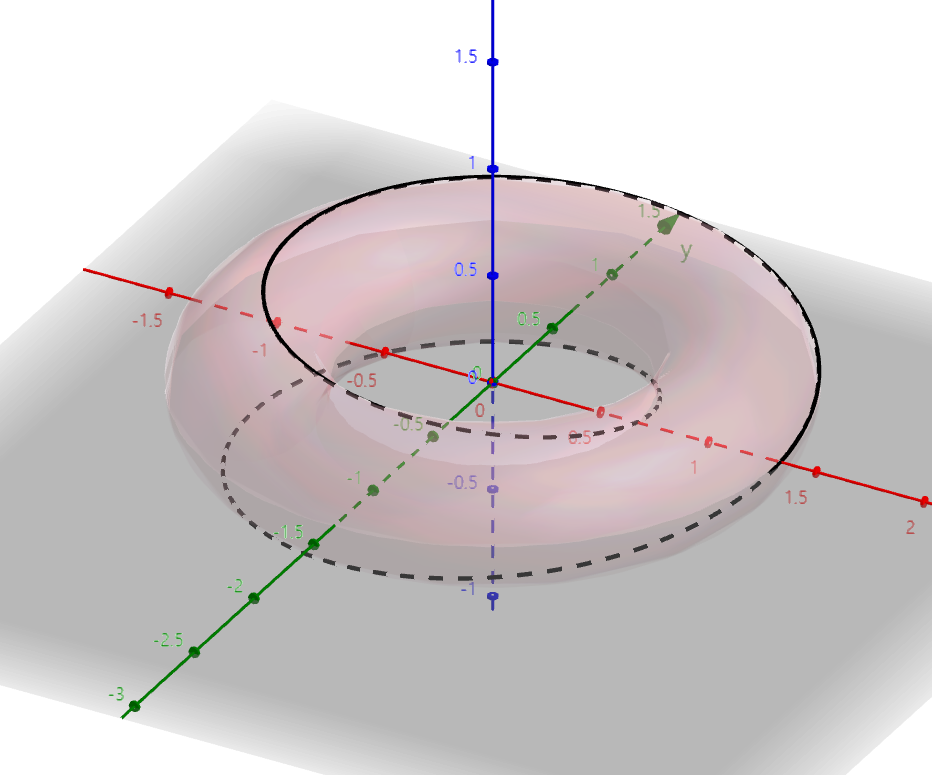
\includegraphics[width=0.9\linewidth]{torus.png}
\captionof{figure}{The path $f$ on the torus $p$}

\begin{exercise}
[Section 54 exersice 6]
Consider the maps $g,h:S^1\to S^1$ given $g(z)=z^n$ and $h(z)=1/z^n$. (Here we represent $S^1$ as the set of complex numbers $z$ of absolute value 1.) Compute the induced homomorphism $g_*$,$h_*$ of the infinite cyclic group $\pi_1(S^1,b_0)$ into itself. [Hint: Recall the equation $(\cos \theta + i\sin \theta)^n = \cos n\theta + \sin n\theta$.]
\end{exercise}
\begin{proof}
Since $S^1$ is path-connected, $\pi_1(S^1,b_0)\cong \pi_1(S^1,(1,0))$. We may assume $b_0=(1,0)$. Let $f:I\to S^1$ given by $f(t)=(\cos 2\pi t, \sin 2\pi t) = e^{2\pi it}$. Then $f(0) = f(1) = (1,0)$, and the equivalence class $[f]\in \pi_1(S^1,(1,0))\cong \mathbb{Z}$ corresponds to $1\in \mathbb{Z}$, so it is a gererater of $\pi_1(S^1,(1,0))$. Define a isomorphism $\phi:\pi_1(S^1,(1,0))\to \mathbb{Z}$ by $\phi([e^{2\pi nt}])=n$. Then $(\phi \circ g_*)([f]) = \phi([g\circ f])=\phi([e^{2\pi nt}])=n$. Since $[f]$ is a generator of $\pi_1(S^1,(1,0))$, $n$ is a generator of $(\phi \circ g_*)(\pi_1(S^1,(1,0)))$, $n \mathbb{Z}$. Consequently, $g_*(\pi_1(S^1,(1,0)))\cong (\phi \circ g_*)(\pi_1(S^1,(1,0))) = n \mathbb{Z}$. Similarly, $h_*(\pi_1(S^1,(1,0))) \cong (\phi \circ h_*)(\pi_1(S^1,(1,0))) = -n \mathbb{Z}$.
\end{proof}

\clearpage

\section{HW2}
$\varnothing$


\end{multicols}
\end{document}

\section{SEQUENCE AND SERIES}

% ---------- ---------- ---------- ---------- ----------
% ---------- ---------- Convergent sequence ---------- ----------
% ---------- ---------- ---------- ---------- ----------
\subsection{Convergent sequence}

\begin{definition}[The definition of convergence of sequences (pma 3.1)]
Let $\{p_n\}$ be a sequence in a metric space $X$.
\begin{enumerate}[label={(\arabic*)}]
\item $\{p_n\}$ is said to \textbf{\textcolor{orange}{converge}} if there is a point $p\in X$ with the following property:
$$ \forall \epsilon>0,\; \exists N\in \mathbb{N}\text{ s.t. }n\geq N\Rightarrow d(p_n,p)<\epsilon$$
In this case, we write $p_n\to p$, or $\lim\limits_{n\to \infty}p_n=p$.
\item The set of all point $p_n$ is called the \textbf{\textcolor{orange}{range}} of the sequence.
\item A sequence is \textbf{\textcolor{orange}{bounded}} if its range is bounded.
\end{enumerate}
\end{definition}

\begin{theorem}[The properties of convergent sequences in metric space (pma 3.2)]
Let $\{p_n\}$ be a sequence in a metric space $X$.
\begin{enumerate}[label={(\alph*)}]
\item The $\{p_n\}$ converges to $p\in X$ \textbf{\emph{if and only if}} every neighborhood of $p$ contains $p_n$ for all but finitely many $n$.
\item If $\{p_n\}$ converges, then its limit is unique.
\item If $\{p_n\}$ converges, then $\{p_n\}$ is bounded.
\item If $E\subset X$ and if $p$ is a limit point of $E$, then there is a sequence $\{p_n\}$ in $E$ such that $p=\lim\limits_{n\to\infty}p_n$.
\end{enumerate}
\end{theorem}
\begin{proof}
\step{b} Given $\epsilon>0$, choose $N>0$ such that $n\geq N$ implies $d(p,p_n)<\frac{\epsilon}{2}$ and $d(p',p_n)<\frac{\epsilon}{2}$. Then $d(p,p')\leq d(p,p_n)+d(p',p_n)<\epsilon$.
\step{c} Given $\epsilon>0$, there exists $N>0$ such that $n\geq N$ implies $d(p,p_n)<\epsilon$. Thus, the range of $\{p_n\}$ is bounded by $\max\{d(p,p_1),d(p,p_2),\dots,d(p,p_{N-1}),\epsilon\}$.
\step{d} Choose $p_n$ such that $d(p,p_n)<\frac{1}{n}$. Given $\epsilon>0$, by Archimedian property, there exists a integer $N$ such that $\frac{1}{N}<\epsilon$. If $n\geq N$, then $d(p,p_n)<\epsilon$.
\end{proof}

% 20240805 #1
\begin{theorem}[Limit operations for complex sequences (pma 3.3)]
Suppose $\{s_n\}$, $\{t_n\}$ are complex sequence, and $s_n\to s$, $t_n\to t$ as $n\to \infty$. Then
\begin{enumerate}[label={(\arabic*)}]
\item $\displaystyle \lim_{n\to \infty}(s_n+t_n)=s+t$.
\item $\displaystyle \lim_{n\to \infty}cs_n=cs$, $\lim_{n\to \infty}(c+s_n)=c+s$ for any number $c$.
\item $\displaystyle \lim_{n\to \infty}(s_nt_n)=st$.
\item $\displaystyle \lim_{n\to \infty}\frac{1}{s_n}=\frac{1}{s}$, provided $s_n\neq 0$ ($n=1,2,\dots$), and $s\neq 0$.
\end{enumerate}
\end{theorem}
% trivial proof

% 20240805 #2
\begin{theorem}[The properties of convergent sequences in Euclidean space (pma 3.4)]
\begin{enumerate}[label={(\alph*)}]
\item[]
\item Suppose $x_n\in \mathbb{R}^k$ ($n=1,2,\dots$) and $x_n=(a_{1,n}, \dots, a_{k,n})$. Then $\{x_n\}\to x=(a_1,\dots,a_k)$ \textbf{\emph{if and only if}} $\lim\limits_{n\to \infty}a_{j,n}=a_j$ ($1\leq j\leq k$).
\item Suppose $\{x_n\}$, $\{y_n\}$ are sequences in $\mathbb{R}^k$, $\{\beta_n\}$ is a sequence of real numbers, and $x_n \to x$, $y_n\to y$, $\beta_n\to \beta$. Then $\lim\limits_{n\to \infty}(x_n+y_n)=x+y$, $\lim\limits_{n\to \infty}x_n\dot y_n=x\dot y$, $\lim\limits_{n\to \infty}\beta_nx_n=\beta x$.
\end{enumerate} 
\end{theorem}
% trivial proof

% ---------- ---------- ---------- ---------- ----------
% ---------- ---------- Subsequences ---------- ----------
% ---------- ---------- ---------- ---------- ----------
\subsection{Subsequences}

\begin{definition}[The definition of subsequences (pma 3.5)]
Given a sequence $\{p_n\}$ , consider a sequence $\{n_k\}$ of positive integer such that $n_1<n_2<\dots$. Then the sequence $\{p_{n_1}\}$ is called a \textbf{\textcolor{orange}{subsequence}} of $\{p_n\}$. If $\{p_{n_i}\}$ converges, its limit is called a \textbf{\textcolor{orange}{subsequential limit}} of $\{p_n\}$.
\end{definition}

% 20240805 #3
\begin{theorem}[\textbf{\textcolor{orange}{Bolzano–Weierstrass theorem}} (pma 3.6)]
\label{thm:bolzano_weierstrass_thm_in_compact_space}
\begin{enumerate}[label={(\alph*)}]
\item[]
\item A sequence in a compact metric space has a subsequences such that converges a point of $X$.
\item Every bounded sequence in $\mathbb{R}^k$ contains a convergent subsequence.
\end{enumerate}
\end{theorem}
\begin{proof}
\step{a} Consider two cases: the range of $\{p_n\}$ is either finite or infinite. The first case is trivial. In the second case, there exists a point $p_{n_k}\in D(p,\frac{1}{k})$ for each $k=1,2,\dots$ (thm \ref{thm:bolzano_weierstrass_thm_in_compact_set}), and it is guaranteed that $n_k\leq n_{k+1}$ (thm \ref{thm:ball_of_limit_pt}).
\step{b} By (a) and thm \ref{thm:bolzano_weierstrass_thm_in_euclidean_set}
\end{proof}

% 20240805 #4
\begin{theorem}
[The set of subsequential limits is closed (pma 3.7)]
\label{thm:subseq_limits_closed}
The subsequential limits of sequence $\{p_n\}$ in a metric space $X$ forms a closed subset of $X$.
\end{theorem}
\begin{hardproof}
Let $E'$ be the set of all subsequential limits of $\{p_n\}$. Suppose $r = d(q,p_{n_1})$, where $q$ is a limit point of $E'$ and $q\neq p_{n_1}$. Then there exist a point $x\in E'$ and a point $p_{n_2}$ such that $d(q,x)<\frac{r}{2^2}$ and $d(x,p_{n_2})<\frac{r}{2^2}$. Consequently, $d(q,p_{n_2})<\frac{r}{2}$. By induction, we can show that $d(q,p_{n_k})<\frac{r}{2^{k-1}}$ for each $k$. Therefore $q\in E'$.
\end{hardproof}

% ---------- ---------- ---------- ---------- ----------
% ---------- ---------- Cauchy sequences ---------- ----------
% ---------- ---------- ---------- ---------- ----------
\subsection{Cauchy sequences}

\begin{definition}
[The definition of Cauchy sequences and diameter (pma 3.8, 3.9)]
Let $X$ be a metric space.
\begin{enumerate}[label={(\arabic*)}]
\item A sequence $\{p_n\}$ in $X$ is said to be a \textbf{\textcolor{orange}{Cauchy sequence}} if $$\forall \epsilon>0, \exists N\in \mathbb{Z}\text{ s.t. }n,m\geq N \Rightarrow d(p_n,p_m)<\epsilon$$
\item Let $E$ be a nonempty subset of $X$, and let $S$ be the set of all real numbers of the form $d(p,q)$, with $p,q\in E$. The $\sup S$ is called the \textbf{\textcolor{orange}{diameter}} of $E$.
\end{enumerate}
If $E_N$ consists of the points $P_N, P_{N+1},\dots$, then $\{p_n\}$ is a Cauchy sequence \textbf{\emph{if and only if}} $\lim\limits_{N\to \infty}\diam E_N=0$.
\end{definition}

% 20240805 #5
\begin{theorem}
[Properties of diameter (pma 3.10)]
Let $X$ be a metric space, let $E\subset X$ be a set, and let $K_n$ be a sequence of compact sets in $X$ such that $K_n\supset K_{n+1}$ for $n=1,2,\dots$.
\begin{enumerate}[label={(\arabic*)}]
\item $\diam \overline{E} = \diam E$
\item If $\lim\limits_{n\to \infty}\diam K_n=0$, then $\bigcap_1^\infty K_n$ consists of exactly one point
\end{enumerate}
\end{theorem}
\begin{proof}
\step{a} Obviously $\diam E < \diam \overline{E}$. On the other hand, for $p,q\in \overline{E}$, there exist $p',q'\in E$ such that $d(p,p')<\epsilon$ and $d(q,q')<\epsilon$. Thus $d(p,q)<2\epsilon + \diam E$.
\end{proof}

% 20240805 #6
\begin{theorem}
[\textbf{\textcolor{orange}{Cauchy criterion}} (pma 3.11)]
\label{thm:cauchy_criterion}
\begin{enumerate}[label={(\alph*)}]
\item[]
\item In any metric space $X$, every convergent sequence is a Cauchy sequence.
\item If $X$ is a compact metric space and if $\{p_n\}$ is a Cauchy sequence in $X$, then $\{p_n\}$ converges to some point of $X$.
\item (Cauchy criterion) In $\mathbb{R}^k$, every Cauchy sequence converges.
\end{enumerate}
\end{theorem}
\begin{hardproof}
\step{b} There exists a subsequence $p_{n_k}\to p$. Given $\epsilon>0$, choose $N_1$ such that $n_k\geq N_1$ implies $d(p_{n_k},p)<\epsilon$, and choose $N_2$ such that $n, n_k\geq N_2$ implies $d(p_n, p_{n_k})<\epsilon$. If $n,n_k\geq \max (N_1, N_2)$, then $d(p_n,p)<2\epsilon$.
\step{c} Let $E_N$ be the set consisting of $p_{N+1},p_{N+2},\dots$ such that $\diam E_N<1$. Then the range of $\{p_n\}$ is bounded by the union of $p_1,p_2,\dots$,$p_N$ and $E_N$. Since a bounded set in $\mathbb{R}^k$ is contained in some $k$-cell, assertion (b) implies (c).
\end{hardproof}

% ---------- ---------- ---------- ---------- ----------
% ---------- ---------- Completeness ---------- ----------
% ---------- ---------- ---------- ---------- ----------
\subsection{Completeness}

\begin{definition}[The definition of completeness (pma 3.12)]
A metric space in which every Cauchy sequence converges is said to be \textbf{\textcolor{orange}{complete}}.
\end{definition}

\begin{remark}
\begin{enumerate}[label={(\arabic*)}]
\item Every compact metric space is complete.
\item Every Euclidean space is complete.
\item Every closed subset of a complete metric space is complete.
\end{enumerate}
\end{remark}

\begin{definition}[The definition of monotone sequences (pma 3.13)]
A sequence $\{s_n\}$ of real numbers is said to be
\begin{enumerate}[label={(\alph*)}]
\item \textbf{\textcolor{orange}{monotonically increasing}} if $s_n\leq s_{n+1}$ for $n=1,2,\dots$.
\item \textbf{\textcolor{orange}{monotonically decreasing}} if $s_n\geq s_{n+1}$ for $n=1,2,\dots$.
\end{enumerate}
\end{definition}

% 20240805 #7

\begin{theorem}
[\textbf{\textcolor{orange}{Monotone Convergence theorem}} (pma 3.14)]
A monotonic sequence converges \textbf{\emph{if and only if}} it is bounded.
\end{theorem}
\begin{proof}
\forward Suppose $s_n\to s$, then $|s - s_n| < 1$ all but finitely many $n$; hence, $\{s_n\}$ is bounded by $\max \{1+s,s_1+s,\dots,s_n+s\}$.
\backward Let $s$ be a least upper bound of $\{s_n\}$ and let $\epsilon>0$ be given. Since $s$ is a least upper bound, there exists some $N$ such that $s-\epsilon < s_N \leq s$. Since $\{s_n\}$ increases, $n\geq N$ implies $s-\epsilon<s_n\leq s$.
\end{proof}

% ---------- ---------- ---------- ---------- ----------
% ---------- ---------- UPPER AND LOWER LIMITS ---------- ----------
% ---------- ---------- ---------- ---------- ----------
\subsection{Upper and lower limits}
\begin{definition}
[Divergence to infinity (pma 3.15)]
If $\forall M\in \mathbb{R}$, $\exists N\in \mathbb{Z}$ such that $n\geq N$ implies $s_n\geq M$, then we write $s_n\to +\infty$. On the other hand, if $s_n\leq M$, then we wirte $s_n\to -\infty$.
\end{definition}

\begin{definition}
[Upper and lower limits (pma 3.16)]
Let $\{s_n\}$ be a sequence of real numbers, and let $E$ be the set of all subsequential limits, including possibly $+\infty, -\infty$. Then $\sup E$ and $\inf E$ are called the \textbf{\textcolor{orange}{upper}} and \textbf{\textcolor{orange}{lower limits}} of $\{s_n\}$; we write $\limsup\limits_{n\to \infty}s_n=\sup E:=s^*$, $\liminf\limits_{n\to \infty}s_n=\inf E:=s_*$.
\end{definition}

% 20240806 #1
\begin{theorem}
[Properties of upper limits (pma 3.17)]
In above definition, $s^*$ has the follwing properties:
\begin{enumerate}[label={(\alph*)}]
\item $s^*\in E$
\item If $x>s^*$, there is an integer $N$ such that $n\geq N$ implies $s_n<x$.
\end{enumerate}
Moreover, $s^*$ is the only number with these properties.
\end{theorem}
\begin{hardproof}
\step{a} If $s^*=+\infty$, then $E$ is not bounded above; hense $s_n$ is not bounded above(thm \ref{thm:bolzano_weierstrass_thm_in_compact_space}), and there exists $\{s_{n_k}\}$ such that $s_{n_k}\to +\infty$. If $s^*$ is real, then (a) follows from thm \Ref{thm:subseq_limits_closed} and thm \Ref{thm:sup_closed_set}. If $s^*=-\infty$, then there is no subsequential limit. Thus $s_n\to -\infty$.
\step{b} If there exists infinitely many $n$ such that $s_n\geq x$, then a number $y\in E$ exists such that $y\geq x>s^*$, leading to a contradiction.
\step{Uniqueness} If $p,q$ satisfy (a) and (b), then we may assume $p<q$. There exists a number $x$ such that $p<x<q$. Since $p$ satisfies (b), $q$ cannnot satisfies (a).
\end{hardproof}

% 20240806 #2
\begin{theorem}
[Condition of convergence (pma 3.16)]
\label{thm:seq_convergence_iff_limsup_liminf}
A real-valued sequence converges \textbf{\emph{if and only if}} its upper limit and lower limit are the same.
\end{theorem}

% 20240806 #3
\begin{example}
[pma 3.20]
Some speical sequences:
\begin{enumerate}[label={(\alph*)}]
\item If $p>0$, then $\lim\limits_{n\to \infty}\frac{1}{n^p}=0$.
\item If $p>0$, then $\lim\limits_{n\to \infty}p^{\frac{1}{n}}=1$.
\item $\lim\limits_{n\to \infty}n^{\frac{1}{n}}=1$.
\item If $p>0$ and $a\in \mathbb{R}$, then $\lim\limits_{n\to \infty}\frac{n^a}{(1+p)^n}=0$.
\item If $|x|<1$, then $\lim\limits_{n\to \infty}x^n=0$.
\end{enumerate}
\end{example}

% ---------- ---------- ---------- ---------- ----------
% ---------- ---------- Series ---------- ----------
% ---------- ---------- ---------- ---------- ----------
\subsection{Series}
\begin{definition}
[pma 3.21]
Let $\{a_k\}$ be a sequence of complex numbers.
\begin{enumerate}[label={(\arabic*)}]
\item $\sum\limits_{k=1}^{\infty}a_k(=\sum a_k)$ is called a(n) \textbf{\textcolor{orange}{(infinite) series}}.
\item $s_n=\sum\limits_{k=1}^{n}a_k$ is called a \textbf{\textcolor{orange}{partial sum}} of the series.
\item If the series converges, then $s=\sum a_k$ is called the sum of the series.
\end{enumerate}
\end{definition}

% 20240806 #4
\begin{theorem}
[pma 3.22]
\label{thm:conv_series}
By Cauchy criterion(thm \Ref{thm:cauchy_criterion}), the series $\sum a_k$ converges \textbf{\emph{if and only if}} for every $\epsilon>0$, there exists an integer $N$ such that $|s_n-s_m|=|\sum_{k=m+1}^{n}a_k|<\epsilon$ whenever $n\geq m\geq N$.
\end{theorem}

% 20240806 #5
\begin{theorem}
[pma 3.23]
\label{thm:conv_series_implies_lim_zero}
If $\sum a_k$ converges, then $\lim_{n\to \infty}a_n = 0$ (taking $m=n$).
\end{theorem}

% 20240806 #6
\begin{theorem}
[pma 3.24]
\label{thm:conv_nonnegative_series}
A series of nonnegative(real) terms converges \textbf{\emph{if and only if}} its partial sums form a bounded sequence.
\end{theorem}

% 20240806 #7
\begin{theorem}
[pma 3.25]
\label{thm:comparison_test}
(Comparison test) If $|a_n|\leq c_n$ for $n>N$ where $N$ is some fixed integer, and if $\sum c_n$ converges, then $\sum a_n$ converges. On the other hand, if $a_n\geq d_n\geq 0$ for $n>N$, and if $\sum d_n$ diverges, then $\sum a_n$ diverges.
\end{theorem}
\begin{proof}
Given $\epsilon>0$, there exists an integer $N'$ such that $n\geq m\geq N'$ implies $\sum_{k=m+1}^{n}c_k < \epsilon$. Then if $n\geq m\geq max(N,N')$, then $|\sum_{k=m+1}^{n}a_k|\leq \sum_{k=m+1}^{n}|a_k|\leq \sum_{k=m+1}^{n}c_k<\epsilon$. The other assertion is derived using similar logic.
\end{proof}

% ---------- ---------- ---------- ---------- ----------
% ---------- ---------- Series of nonnegative terms ---------- ----------
% ---------- ---------- ---------- ---------- ----------
\subsection{Series of nonnegative terms}

% 20240806 #8
\begin{theorem}
[pma 3.26]
\textbf{(Geometric Series)} If $0\leq x< 1$, then $\sum x^n=\frac{1}{1-x}$. If $x\geq 1$, the series diverges.
\end{theorem}
\begin{proof}

\end{proof}

% 20240806 #9
\begin{theorem}
[pma 3.27]
Suppose $a_1\geq a_2\geq \dots \geq 0$. Then $\sum a_n$ converges \textbf{\emph{if and only if}} $\sum 2^ka_{2^k}$ converges.
\end{theorem}
\begin{proof}

\end{proof}

% 20240807 #1 : trivial
\begin{theorem}
[pma 3.28]
$\sum \frac{1}{n^p}$ converges if $p>1$ and diverges if $p\leq 1$.
\end{theorem}

% 20240807 #2 : trivial
\begin{theorem}
[pma 3.29]
$\sum\limits_{n=2}^{\infty}\frac{1}{n(\log n)^p}$ converges if $p>1$ and diverges if $p\leq 1$.
\end{theorem}

% ---------- ---------- ---------- ---------- ----------
% ---------- ---------- The number e ---------- ----------
% ---------- ---------- ---------- ---------- ----------
\subsection{The number e}
\begin{definition}
[pma 3.30]
$e=\sum\limits_{n=0}^\infty \frac{1}{n!}$.
\end{definition}

% 20240807 #3 : non-trivial
\begin{theorem}
[pma 3.31]
$\lim\limits_{n\to \infty}(1+\frac{1}{n})^n=e$.
\end{theorem}
\begin{hardproof}
Let $s_n=\sum_{k=0}^n\frac{1}{k!}$, $t_n=(1+\frac{1}{n})^n$. Then $t_n=1+1+\frac{1}{2!}(1-\frac{1}{n})+\frac{1}{3!}(1-\frac{1}{n})(1-\frac{2}{n})+\dots+\frac{1}{n!}(1-\frac{1}{n})(1-\frac{2}{n})\dots(1-\frac{n-1}{n})$. Hense $t_n\leq s_n$, so that $\limsup_{n\to \infty}t_n\leq e$. Next, if $n\geq m$, $t_n\geq 1+1+\frac{1}{2!}(1-\frac{1}{n})+\dots+\frac{1}{m!}(1-\frac{1}{n})\dots(1-\frac{m-1}{n})$. Let $n\to \infty$, keeping $m$ fixed. We get $\liminf_{n\to \infty}t_n\geq 1+1+\frac{1}{2!}+\dots+\frac{1}{m!}$, so that $s_m\leq \liminf_{n\to \infty} t_n$. Letting $m\to \infty$, we finally get $e\leq \liminf_{n\to \infty}t_n$.
\end{hardproof}

\begin{remark}
[pma 3.32]
$e-s_n=\frac{1}{(n+1)!}+\frac{1}{(n+2)!}+\dots<\frac{1}{(n+1)!}\{1+\frac{1}{n+1}+\frac{1}{(n+1)^2}+\dots\}=\frac{1}{n!n}$.
\end{remark}

% 20240807 #4
\begin{theorem}
[pma 3.32]
$e$ is irrational.
\end{theorem}
\begin{hardproof}
Suppose $e=p/q$. Then $0<q!(e-s_q)<1/q$. By our assumption, $q!(e-s_q)$ is an integer, leading to a contradiction.
\end{hardproof}

% ---------- ---------- ---------- ---------- ----------
% ---------- ---------- The root and ratio tests ---------- ----------
% ---------- ---------- ---------- ---------- ----------
\subsection{The root and ratio tests}

\begin{mytheorem}
[Root test]
\label{thm:root_test}
Given $\sum a_n$, put $\alpha = \limsup\limits_{n\to \infty}|a_n|^{\frac{1}{n}}$. Then
\begin{enumerate}[label={(\alph*)}]
\item if $\alpha < 1$, $\sum a_n$ converges;
\item if $\alpha > 1$, $\sum a_n$ diverges;
\item if $\alpha = 1$, the test gives no information.
\end{enumerate}
\end{mytheorem}
\begin{proof}
[PMA 3.33] (a) If $\alpha < \beta < 1$, the comparison test show the convergence of $\sum a_n$. \\
(b) If $\alpha > 1$, by the definition of limsup, there exist infinitely many $n$ such that $|a_n|>1$, so that the condition $a_n\to 0$(necessaty for convergence of $\sum a_n$) does not hold.
\end{proof}

\begin{mytheorem}
[Raito test]
\label{thm:ratio_test}
The series $\sum a_n$
\begin{enumerate}[label={(\alph*)}]
\item converges if $\limsup\limits_{n\to \infty}|\frac{a_{n+1}}{a_n}|<1$,
\item divergess if $|\frac{a_{n+1}}{a_n}|\geq 1$ for all $n\geq n_0$, where $n_0$ is some fixed integer.
\end{enumerate}
\end{mytheorem}
\begin{proof}
[PMA 3.34]
(a) Suppose for some $N\in \mathbb{Z}$, $\displaystyle \left|\frac{a_{n+1}}{a_n}\right|<\beta<1$ for $n\geq N$. Then $|a_{N+p}|<\beta|a_{N+p-1}|<\dots<\beta^p|a_N|$. If we set $n=N+p$, then $|a_n|<|a_N|\beta^{n-N}$ for $n\leq N$, and $\sum a_n$ converges by the comparison test.
\end{proof}

\begin{myproposition}
For any sequence $\{c_n\}$ of positive numbers,
$$\liminf_{n\to \infty}\frac{c_{n+1}}{c_n}\leq \liminf_{n\to \infty}\sqrt[n]{c_n},$$
$$\limsup_{n\to \infty}\sqrt[n]{c_n}\leq \limsup_{n\to \infty}\frac{c_{n+1}}{c_n}$$
\end{myproposition}
\begin{proof}
[pma 3.37]
\end{proof}

% ---------- ---------- ---------- ---------- ----------
% ---------- ---------- Power series ---------- ----------
% ---------- ---------- ---------- ---------- ----------
\subsection{Power series}
\begin{definition}
[pma 3.38]
Given a sequence $\{c_n\}$ of complex numbers, the series
$$\sum_{n=0}^{\infty}c_nz^n$$
is called a \textbf{\textcolor{orange}{power series}}. The numbers $c_n$ are called the \textbf{\textcolor{orange}{coefficient}} of the series; $z$ is a complex number.
\end{definition}

% 20240809 #2
\begin{theorem}
[pma 3.39]
Put $$\alpha =\limsup_{n\to \infty}\sqrt[n]{|c_n|},\;\;R=\frac{1}{\alpha}$$
Then $\sum c_nz^n$ converges if $|z|<R$ and diverges if $|z|>R$.
\end{theorem}


% ---------- ---------- ---------- ---------- ----------
% ---------- ---------- Summation by parts ---------- ----------
% ---------- ---------- ---------- ---------- ----------
\subsection{Summation by parts}

% 20240809 #3
\begin{theorem}
[pma 3.41]
Given two sequence $\{a_n\}$, $\{b_n\}$, put $A_n=\sum\limits_{k=0}^{n}a_k$ if $n\geq 0$; put $A_{-1}=0$. Then, if $0\leq p\leq q$, we have
$$\sum_{n=p}^qa_nb_n=\sum_{n=p}^{q-1}A_n(b_n-b_{n+1})+A_qb_q-A_{p-1}b_p$$
\end{theorem}
\begin{proof}
Computation.
\end{proof}

% 20240809 #4
\begin{theorem}
[pma 3.42]
Suppose
\begin{enumerate}[label={(\alph*)}]
\item $A_n$ form a bounded sequence;
\item $b_0\geq b_1\geq \dots$;
\item $\lim\limits_{n\to \infty}b_n=0$.
\end{enumerate}
Then $\sum a_nb_n$ converges.
\end{theorem}
\begin{proof}

\end{proof}

% 20240809 #5
\begin{corollary}
[pma 3.43]
Suppose
\begin{enumerate}[label={(\alph*)}]
\item $|c_1|\geq |c_2|\geq \dots$;
\item $c_{2m-1}\geq 0$, $c_{2m}\leq 0$ for $m=1,2,\dots$;
\item $\lim\limits_{n\to \infty}c_n=0$.
\end{enumerate}
Then $\sum c_n$ converges.    
\end{corollary}

% 20240809 #6
\begin{theorem}
[pma 3.44]
Suppose
\begin{enumerate}[label={(\alph*)}]
\item the radius of convergence of $\sum c_nz^n$ is 1;
\item $c_0\geq c_1\geq \dots$;
\item $\lim\limits_{n\to \infty}c_n=0$.
\end{enumerate}
Then $\sum c_nz^n$ converges at every point on the circle $|z|=1$, except possibly at $z=1$.
\end{theorem}
\begin{proof}

\end{proof}

% ---------- ---------- ---------- ---------- ----------
% ---------- ---------- Absolute convergence ---------- ----------
% ---------- ---------- ---------- ---------- ----------
\subsection{Absolute convergence}

\begin{definition}
[pma 3.45]
The series $\sum a_n$ is said to \textbf{\textcolor{orange}{converge absolutely}} if the series $\sum |a_n|$ converges.
\end{definition}

% 20240809 #7
\begin{theorem}
[pma 3.45]
If $\sum a_n$ converges absolutely, then $\sum a_n$ converges.
\end{theorem}

% ---------- ---------- ---------- ---------- ----------
% ---------- ---------- Addition and multiplication of series ---------- ----------
% ---------- ---------- ---------- ---------- ----------
\subsection{Addition and multiplication of series}

% 20240809 #8
\begin{theorem}
[pma 3.47]
If $\sum a_n=A$, and $\sum b_n=B$, then $\sum (a_n+b_n) = A+B$, and $\sum ca_n = cA$, for any fixed $c$.
\end{theorem}

\begin{definition}
[pma 3.48]
Given $\sum a_n$ and $\sum b_n$, we put
$$ c_n=\sum_{k=0}^{n}a_kb_{n-k}\;\; (n=0,1,\dots)$$
and call $\sum c_n$ the \textbf{\textcolor{orange}{product}} of two given series, in other word, the \textbf{\textcolor{orange}{Cauchy product}}  (consider the equation $(a_0+a_1z+a_2z^2+\dots)(b_0+b_1z+b_2z^2+\dots)=a_0b_0+(a_0b_1+a_1b_0)z+(a_0b_2+a_1b_1+a_2b_0)z^2+\dots$).
\end{definition}

\begin{example}
[pma 3.49]
A counterexample to the assertion that the Cauchy product of two convergent series converges:
$$A_n=\sum_{n=0}^\infty \frac{(-1)^n}{\sqrt{n+1}}$$
Consider the Cauchy product of $A_n$ itself:
$$c_n=(-1)^n\sum_{k=0}^n\frac{1}{\sqrt{(n-k+1)(k+1)}}$$
Since
$$(n-k+1)(k+1)=(\frac{n}{2}+1)^2-(\frac{n}{2}-k)^2\leq (\frac{n}{2}+1)^2$$
we have
$$|c_n|\geq \sum_{k=0}^n \frac{2}{n+2}=\frac{2(n+1)}{n+2}$$
\end{example}

% 20240810 #1
\begin{theorem}
[pma 3.50]
If $\sum a_n$ converges absolutely, $\sum a_n=A$, $\sum b_n=B$, then the Cauchy product $\sum c_n=AB$.
\end{theorem}
\begin{hardproof}

\end{hardproof}

% 20240810 #2
\begin{theorem}
[pma 3.51]
If the series $\sum a_n$, $\sum b_n$, $\sum c_n$ converge to $A$, $B$, $C$, then $C=AB$.
\end{theorem}
\begin{proof}
Latter
\end{proof}

% ---------- ---------- ---------- ---------- ----------
% ---------- ---------- Rearrangements ---------- ----------
% ---------- ---------- ---------- ---------- ----------
\subsection{Rearrangements}

\begin{definition}
[pma 3.52]
Let $\{k_n\}$ be a 1-1 function from $\mathbb{N}$ to $\mathbb{N}$. Putting $a'_n=a_{k_n}$, we say that $\sum a_n'$ is a \textbf{\textcolor{orange}{rearrangement}} if $\sum a_n$.
\end{definition}


% 20240810 #3
\begin{theorem}
[pma 3.54]
Let $\sum a_n$ be a series of real numbers which converges, but not absolutely. Suppose $-\infty\leq \alpha\leq \beta\leq \infty$. Then there exists a rearrangement $\sum a_n'$ with partial sums $s_n'$ such that $\liminf\limits_{n\to \infty}s_n'=\alpha$, $\limsup\limits_{n\to \infty}=\beta$.
\end{theorem}
\begin{hardproof}

\end{hardproof}

% 20240810 #4
\begin{theorem}
[pma 3.55]
If $\sum a_n$ is a series of complex numbers which converges absolutely, then everyy rearrangement of $\sum a_n$ converges,and they all converge to the same sum.
\end{theorem}
\begin{hardproof}

\end{hardproof}

\clearpage
\section{CONTINUITY}
% ---------- ---------- ---------- ---------- ----------
% ---------- ---------- LIMITS OF FUNCTIONS ---------- ----------
% ---------- ---------- ---------- ---------- ----------
\subsection{LIMITS OF FUNCTIONS}

\begin{definition}
Suppose $X$ and $Y$ are metric spaces, $E\subset X$, $p\in E'$, $f:E\to Y$.
Then we write $\lim\limits_{x\to p}f(x)=q$ if there is a point $q\in Y$ with following property:
$$\forall \epsilon>0,\; \exists \delta>0 \text{ s.t. } x\in E\land d_X(x,p)<\delta \Rightarrow d_Y(f(x),q)<\epsilon$$
\end{definition}

\begin{theorem}
$\lim\limits_{x\to p}f(x)=q$ \textbf{\emph{if and only if}} $\lim\limits_{n\to \infty}f(p_n)=q$ for every sequence $\{p_n\}$ in $E$ such that $p_n\neq p$ and $\lim\limits_{n\to \infty}p_n=p$.
\end{theorem}
\begin{proof}
\forward Given $\epsilon>0$, there exists $\delta>0$ such that $d_Y(f(x),q)<\epsilon$ if $x\in E$ and $0<d_X(x,p)<\delta$. Also, there exists $N$ such that $n>N$ implies $0<d_X(p_n,p)<\delta$.
\backward Suppose, for contradiction, that there exists an $\epsilon>0$ such that for every $\delta>0$ there exists a point $x_\delta\in E$, for which $d_Y(f(x_\delta),q)\geq \epsilon$ but $0<d_X(x_\delta,p)<\delta$. Take $\delta_n = 1/n$.
\end{proof}

\begin{corollary}
If $f$ has a limit at $p$, this limit is unique.
\end{corollary}

\begin{theorem}
Suppose $f,g$ are complex functions on $E$, and $\lim\limits_{x\to p}f(x)=A$, $\lim\limits_{x\to p}g(x)=B$. Then
\begin{enumerate}[label={(\alph*)}]
\item $\lim\limits_{x\to p}(f+g)(x) = A+B$;
\item $\lim\limits_{x\to p}(fg)(x) = AB$;
\item $\lim\limits_{x\to p}(\frac{f}{g})(x)=\frac{A}{B}$, if $B\neq 0$.
\end{enumerate}
\end{theorem}

% ---------- ---------- ---------- ---------- ----------
% ---------- ---------- CONTINUOUS FUNCTIONS ---------- ----------
% ---------- ---------- ---------- ---------- ----------
\subsection{CONTINUOUS FUNCTIONS}

\begin{definition}
Suppose $X$ and $Y$ are metric space, $E\subset X$, $p\in E$, and $f:E\to Y$. Then $f$ is said to be \textbf{\textcolor{orange}{continuous at $p$}} if
$$ \forall \epsilon>0,\exists \delta>0 \forall x\in E:d_X(x,p)<\delta \Rightarrow d_Y(f(x),f(p))<\epsilon$$
\end{definition}

\begin{theorem}
Assume also that $p\in E\cap E'$. Then $f$ is continuous at $p$ \textbf{\emph{if and only if}} $\lim\limits_{x\to p}f(x)=f(p)$.
\end{theorem}

\begin{theorem}
Suppose $X$, $Y$, $Z$ are metric space, $E\subset X$, $f:E\to Y$, $g:f(X)\to Z$, and $h: E\to Z$ given by $h(x)=g(f(x))$ for $x\in E$. If $f$ is continuous at $p\in E$ and $g$ is continuous at $f(p)$, then $h$ is continuous at $p$. $h$ is called the \textbf{\textcolor{orange}{composition}} or \textbf{\textcolor{orange}{composite}} of $f$ and $g$. We write $h = g\circ f$.
\end{theorem}
\begin{proof}
Given $\epsilon>0$, since $g$ is continuous at $f(p)$, $\exists \eta>0$ s.t. $y\in f(E)\land d_Y(y,f(p))<\eta \Rightarrow d_Z(g(y),g(f(p)))<\epsilon$. Since $f$ is continuous at $p$, $\exists \delta>0$ s.t. $x\in E\land d_X(x,p)<\delta \Rightarrow d_Y(f(x),f(p))<\eta$.
\end{proof}

\begin{theorem} \label{thm:equivalent_definition_of_continuity}
$f:X\to Y$ is a \textbf{\textcolor{orange}{continuous on $X$}} \textbf{\emph{if and only if}} $f^{-1}(V)$ is open in $X$ for every open set $V$ in $Y$.
\end{theorem}
\begin{proof}
\forward Suppose $p\in E$ and $f(p)\in V\subset Y$. Since $V$ is open, there exists $\epsilon >0$ s.t. $D_Y(f(p),\epsilon)\subset V$. Also, by definition of continuity, there exists $\delta>0$ s.t. $x\in X\land d_X(x,p)<\delta$ implies $d(f(x),f(p))< \epsilon$. Thus $D_X(p,\delta)\subset f^{-1}(V)$, i.e. $p$ is an interior point.
\backward Given $p\in X$ and $\epsilon>0$, let $V=D_Y(f(p),\epsilon)$. Then $V$ is open in $Y$; hence $f^{-1}(V)$ is open; hence there exists $\delta>0$ such that $(D_X(p,\delta)\cap X)\subset f^{-1}(V)$.
\end{proof}

\begin{corollary}
$f$ is continuous \textbf{\emph{if and only if}} $f^{-1}(C)$ is closed in $X$ for every closed set $C$ in $Y$. (Consider that $f^{-1}(E^c)=[f^{-1}(E)]^c$)
\end{corollary}

\begin{theorem}
Let $f$ and $g$ be complex continuous functions on a metric space $X$. Then $f+g$, $fg$, $f/g$ are continuous.
\end{theorem}

\begin{theorem}
\begin{enumerate}[label={(\alph*)}]
\item Let $f_1,\dots,f_k$ be real functions on a metric space $X$, and let $f$ be the mapping of $X$ into $\mathbb{R}^k$ defined by $f(x)=(f_1(x),\dots, f_k(x))$. Then $f$ is continuous \textbf{\emph{if and only if}} each of the functions $f_1,\dots,f_k$ is continuous.
\item If $f$ and $g$ are continuous mapping on $X$ into $\mathbb{R}^k$, then $f+g$ and $f\dot g$ are continuous on $X$.
\end{enumerate}
\end{theorem}
\begin{proof}
\step{a} 
\forward $|f_j(x)-f_j(y)| \leq |f(x)-f(y)|$
\backward Given $x_0\in X$ and $\epsilon>0$, choose $\delta>0$ s.t. $d(x_0,x)<\delta$ implies $d(f_j(x_0), f_j(x))< \epsilon / \sqrt{k}$ for $j=1,\dots, k$.
\end{proof}

% ---------- ---------- ---------- ---------- ----------
% ---------- ---------- CONTINUITY AND COMPACTNESS ---------- ----------
% ---------- ---------- ---------- ---------- ----------
\subsection{CONTINUITY AND COMPACTNESS}

\begin{definition}
$f:E\to \mathbb{R}^k$ is said to \textbf{\textcolor{orange}{bounded}} if there is a real number $M$ such that $|f(x)|\leq M$ for all $x\in E$.
\end{definition}

\begin{theorem}
Let $X$ be a compact metric space, $Y$ a metric space, $f:X\to Y$ continuous. Then $f(X)$ is compact.
\end{theorem}
\begin{proof}
Let $\{V_n\}$ be an open cover of $f[X]$. Then $f^{-1}[V_n]$ is open in $X$; hence there exists a subcover $\{f^{-1}[V_{n_\alpha}]\}$ that covers $X$. Since $f[f^{-1}[E]]\subset E$ for every $E\subset Y$, the assertion holds.
\end{proof}

\begin{theorem}
Let $X$ be a compact metric space and suppose $f:X\to \mathbb{R}^k$ be a continuous function. Then $f[X]$ is closed and bounded, meaning that $f$ is bounded.
\end{theorem}

\begin{theorem}
Let $X$ be a compact metric space and suppose $f:X\to \mathbb{R}$ be a continuous function. Then there exist the \textbf{\textcolor{orange}{maximum}} point $p$ and \textbf{\textcolor{orange}{minimum}} point $q$ in $X$ such that $f(q)\leq f(x)\leq f(p)$ for all $x\in X$.
\end{theorem}

\begin{theorem}
Let $X$ be a compact metric space, $Y$ a metric space, and $f:X\to Y$ a continuous bijection. Then the \textbf{\textcolor{orange}{inverse map}} $f^{-1}:Y\to X$, defined by $f^{-1}(f(x))=x$ for $x\in X$, is continuous.
\end{theorem}
\begin{proof}
Let $V$ be an open set in $X$, then $V^c$ is compact, and so is $f[V^c]$. Since $f[V]=(f[V^c])^c$, $f[V]$ is open. By theorem \Ref{thm:equivalent_definition_of_continuity}, the assertion holds.
\end{proof}

\begin{definition}
Let $X$ and $Y$ be metric spaces. We say $f:X\to Y$ \textbf{\textcolor{orange}{uniformly continuous}} on $X$ if
$$\forall \epsilon>0,\exists \delta>0,\forall p,q\in X:d_X(p,q)<\delta \Rightarrow d_Y(f(p),f(q))<\epsilon$$
\end{definition}

\begin{theorem}
Let $X$ be a compact metric space, $Y$ a metric space, $f:X\to Y$ a continuous function. Then $f$ is uniformly continuous on $X$.
\end{theorem}
\begin{proof}
Given $\epsilon>0$, for each $p\in X$ there exists $\delta_p>0$ such that $q\in X$, $d_X(p,q)<\delta_p$ implies $d_Y(f(p),f(q))<\frac{1}{2}\epsilon$. Since the collection $\{D(p,\frac{1}{2}\delta_p)\}$ is an open cover of $X$, there exists a finite subcover $\{D(p_n,\frac{1}{2}\delta_{p_n})\}$. Put $\delta = \frac{1}{2}\min \{D(p_n,\delta_{p_n}/2)\}$. Let $p,q\in X$ such that $d_X(p,q)<\delta$. Then there exists $1\leq m\leq n$ such that $p\in D(p_m,\frac{1}{2}\delta_{p_m})$, which implies $d_X(q,p_m)\leq d_X(p,q)+d_x(p,p_m)<\delta+\frac{1}{2}\delta_{p_m}\leq \delta_{p_m}$. Finally, $d_Y(f(p),f(q))\leq d_Y(f(p),f(p_m))+d_Y(f(p_m),f(q))<\epsilon$.
\end{proof}

\begin{theorem}
Let $E$ be a noncompact set in $\mathbb{R}$. Then
\begin{enumerate}[label={(\alph*)}]
\item there exists a continuous function on $E$ which is not bounded;
\item there exists a continuous and bounded function on $E$ which has no maximum;
\item if $E$ is bounded, then there exists a continuous function on $E$ which is not uniformly continuous
\end{enumerate}
\end{theorem}
\begin{proof}
If $E$ is bounded, there exists a point $x_0\in E'\backslash E$. 
\step{a} ($E$ bounded) $f(x)=\frac{1}{x-x_0}$; (unbounded) $f(x)=x$.
\step{b} ($E$ bounded) $f(x)=\frac{1}{1+(x-x_0)^2}$; (unbounded) $f(x)=\frac{x^2}{1+x^2}$
\step{c} The first function in (a).
\end{proof}

% ---------- ---------- ---------- ---------- ----------
% ---------- ---------- CONTINUITY AND CONNECTEDNESS ---------- ----------
% ---------- ---------- ---------- ---------- ----------
\subsection{CONTINUITY AND CONNECTEDNESS}
\begin{theorem}
Let $X,Y$ be metric spaces, $f:X\to Y$ a continuous map. If $E\subset X$ is connected, the $f[E]$ is connected.
\end{theorem}
\begin{proof}
Let $Y_1$, $Y_2$ be sets which seperate $f[E]$. Then clearly $X_1\subset f^{-1}[Y_1]$, and since $f$ is continuous and $f^{-1}[\overline{Y_1}]$ is closed, $\overline{X_1}\subset f^{-1}[\overline{Y_1}]$. Therefore, $\overline{Y_1}\cap Y_2=\emptyset$ implies $\overline{X_1}\cap X_2=\emptyset$. Similary, $X_1\cap \overline{X_2}=\emptyset$, leading to a contradiction.
\end{proof}

\begin{corollary}
(\textbf{\emph{Intermediate value theorem}}) Let $f:[a,b]\to \mathbb{R}$ be continuous. Then $f$ has the \textbf{\textcolor{orange}{intermediate value property}}: If $f(a)<c<f(b)$, then there exists a point $x\in(a,b)$ such that $f(x)=c$.
\end{corollary}


% ---------- ---------- ---------- ---------- ----------
% ---------- ---------- DISCONTINUITIES ---------- ----------
% ---------- ---------- ---------- ---------- ----------
\subsection{DISCONTINUITIES}

\begin{definition}
Let $f:(a,b)\to (a,b)$, $a\leq x<b$, and $\{t_n\}$ a sequence in $(x,b)$ such that $t_n\to x$. If $f(t_n)\to q$ as $t_n\to x$, then we write $f(x+)=q$. 
\end{definition}

\begin{definition}
Suppose $f$ is discontinuous at a point $x$. If $f(x+)$ and $f(x-)$ exist, then $f$ is said to have a discontinuity of the \textbf{\textcolor{orange}{first kind}}, or a \textbf{\textcolor{orange}{simple discontinuity}} at $x$. Otherwise the discontinuity is said to be of the \textbf{\textcolor{orange}{second kind}}.
\end{definition}

% ---------- ---------- ---------- ---------- ----------
% ---------- ---------- MONOTONIC FUNCTIONS ---------- ----------
% ---------- ---------- ---------- ---------- ----------
\subsection{MONOTONIC FUNCTIONS}
\begin{definition}
Let $f$ be real on $(a,b)$. Then $f$ is said to be \textbf{\textcolor{orange}{monotonically increasing}} on $(a,b)$ if $a<x<y<b$ implies $f(x)\leq f(y)$.
\end{definition}

\begin{theorem}
Let $f$ be monotonically inceasing on $(a,b)$. Then for every point $x\in (a,b)$, $\sup\limits_{a<t<x}f(t)=f(x-)\leq f(x)\leq f(x+)=\inf\limits_{x<t<b}f(t)$. Furthermore, if $a<x<y<b$, then $f(x+)\leq f(y-)$.
\end{theorem}
\begin{proof}
Let $A=\sup_{a<t<x}f(t)$. Given $\epsilon>0$, there exists $\delta>0$ such that $A-\epsilon<f(x-\delta)\leq A$. Since $f$ is monotonic, it follows that $A-\epsilon<f(x-\delta)\leq f(t)\leq A$ for $x-\delta<t<x$, i.e., $0<f(t)-A<\epsilon$. The second half of the statement holds since $f(x+) = \inf_{x<t<y}f(t)\leq \sup_{x<t<y}f(t)=f(y-)$.
\end{proof}

\begin{corollary}
Monotonic functions have no discontinuities of the seconed kind.
\end{corollary}

\begin{theorem}
Let $f$ be monotonic on $(a,b)$. Then the set of points of $(a,b)$ at which $f$ is discontinuous is at most countable.
\end{theorem}
\begin{proof}
Let $E$ be the set of points at which $f$ is discontinuous. Then for each $x\in E$, there exists a rational number $r_x$ such that $f(x-)<r_x<f(x+)$. Since $x_1<x_2\Rightarrow f(x_1+)\leq f(x_2-)$, we see that $r_{x_1}\neq r_{x_2}$ whenever $x_1\neq x_2$. Therefore, we have a bijective mapping between $E$ and the set $\{r_x\}$.
\end{proof}

\begin{example}
Let $\{c_n\}$ be a set of positive numbers which $\sum c_n$ converges, $E$ the set of rational number in $(a,b)$ arranged in $\{x_n\}$, and $f(x)=\sum\limits_{x_n<x}c_n$ for $a<x<b$. Then
\begin{enumerate}[label={(\arabic*)}]
\item $f$ is monotonically increasing on $(a,b)$;
\item $f$ is discontinuous at every point of $E$;
\item $f$ is continuous at every point of $E^c$.
\end{enumerate}
\end{example}
\begin{proof}
\step{2} $f(x_n+)-f(x_n-)=c_n$.
\step{3} Given $\epsilon>0$ and $x\in E^c$, choose $N\in \mathbb{Z}^+$ such that $\sum\limits_{n=N+1}^\infty < \epsilon$. Let $\delta = \min \{|x-x_n|:1\leq n\leq N\}$ ($\delta>0$ because $x\in E^c$). Then $|x-y|<\delta$ implies $|f(x)-f(y)|\leq \sum_{n=N+1}^\infty c_n<\epsilon$ (if $|x-y|<\delta$, then $x_n$ does not lies in the interval $x$ and $y$, i.e., $c_n$ does not appear in the difference).
\end{proof}

% ---------- ---------- ---------- ---------- ----------
% ---------- ---------- INFINITE LIMITS AND LIMITS AT INFINITY ---------- ----------
% ---------- ---------- ---------- ---------- ----------
\subsection{INFINITE LIMITS AND LIMITS AT INFINITY}
\begin{notebox}
The concept of 'neighborhood' is extended to infinity, but I am not sure where it is applied.
\end{notebox}

\begin{definition}
For any $c\in \mathbb{R}$, $(c,+\infty)$ is a neighborhood of $+\infty$. The same applies to $-\infty$.
\end{definition}

\begin{definition}
$f(t)\to A$ as $t\to x$ where $A$ and $x$ are in the extended real number system, if for every neighborhood $U$ of $A$, there is a neighborhood $V$ of $x$ such that $V\cap E$ is not empty and $f(t)\in U$ for all $t\in V\cap E$, $t\neq x$.
\end{definition}

\clearpage
\section{DIFFERENTIATION}
% ---------- ---------- ---------- ---------- ----------
% ---------- ---------- REARRANGEMENTS ---------- ----------
% ---------- ---------- ---------- ---------- ----------
\begin{notebox}
2024-08-16: only def and thm : have to pf
\end{notebox}
\subsection{REARRANGEMENTS}

\begin{definition}
Let $f:[a,b]\to \mathbb{R}$. $\displaystyle f'(x)=\lim_{t\to x}\frac{f(t)-f(x)}{t-x}$ for any $x\in [a,b]$. $f'$ is called the \textbf{\textcolor{orange}{derivative}} of $f$, and $f$ is \textbf{\textcolor{orange}{differentiable}} at a point $x$ if $f'$ is defined at $x$.
\end{definition}

\begin{theorem}
Differentiability implies continuity.
\end{theorem}
\begin{proof}

\end{proof}

\begin{theorem}
If $f,g$ differentiable at $x$,
\begin{enumerate}[label={(\alph*)}]
\item $(f+g)'(x) = f'(x) + g'(x)$;
\item $(fg)'(x) = (f'g)(x) + (fg')(x)$;
\item $\displaystyle \left(\frac{f}{g}\right)'(x) =  \frac{(f'g)(x)-(fg')(x)}{g^2(x)}$ if $g'(x)\neq x$
\end{enumerate} 
\end{theorem}
\begin{proof}

\end{proof}

\begin{theorem}
(Chain rule) Let $f$ be a continuous function on $[a,b]$, $I$ a interval containing $[a,b]$, $g$ a function defined on $I$. Suppose $f'(x)$ exists at some point $x\in [a,b]$, and $g'(f(x))$ exists. If $h(t) = g(f(t))$ for $a\leq t\leq b$, then $h$ is differentiable at $x$, and $h'(x) = g'(f(x))f'(x)$.
\end{theorem}
\begin{proof}

\end{proof}

% ---------- ---------- ---------- ---------- ----------
% ---------- ---------- MEAN VALUE THEOREMS ---------- ----------
% ---------- ---------- ---------- ---------- ----------
\subsection{MEAN VALUE THEOREM}
\begin{definition}
Let $f$ be a real function defined on a metric space $X$. We say $f$ has a \textbf{\textcolor{orange}{local maximum}} at a point $p\in X$ if there exists $\delta>0$ such that $f(q)\leq f(p)$ for all $q\in X$ with $d(p,q)<\delta$.
\end{definition}

\begin{theorem}
Let $f$ be defined on $[a,b]$. If $f$ has a local maximum at a point $x\in(a,b)$ and if $f'(x)$ exists, then $f'(x)=0$.
\end{theorem}
\begin{proof}

\end{proof}

\begin{theorem}
(Cauchy mean value theorem) If $f,g$ be continuous real functions on $[a,b]$ which are differentiable in $(a,b)$, then there is a point $c\in (a,b)$ at which $[f(b)-f(a)]g'(c)=[g(b)-g(a)]f'(c)$.
\end{theorem}
\begin{proof}
Put $h(t)=[f(b)-f(a)]g(t)-[g(b)-g(a)]f(t)$ for $a\leq t\leq b$.
\end{proof}

\begin{corollary}
(Mean value theorem) If $g(x)=x$, there exists a point $c\in (a,b)$ at which $f(b)-f(a)=(b-a)f'(c)$.
\end{corollary}

\begin{theorem}
Suppose $f$ is differentiable in $(a,b)$.
\begin{enumerate}[label={(\alph*)}]
\item If $f'(x)\geq 0$ for all $x\in(a,b)$, then $f$ is monotonically increasing.
\item If $f'(x)=0$ for all $x\in (a,b)$, then $f$ is constant.
\item If $f'(x)\leq 0$ for all $x\in (a,b)$, then $f$ is monotonically decreasing.
\end{enumerate}
\end{theorem}
\begin{proof}
For $a< x_1< x_2< b$, there is a point $x\in (x_1,x_2)$ such that $f(x_2)=f(x_1)=(x_2-x_1)f'(x)$.
\end{proof}

% ---------- ---------- ---------- ---------- ----------
% ---------- ---------- THE CONTINUITY OF DERIVATIVES ---------- ----------
% ---------- ---------- ---------- ---------- ----------
\subsection{THE CONTINUITY OF DERIVATIVES}

\begin{theorem}
(\textbf{\emph{Darboux's theorem}}) Let $I$ be a closed interval, $f:I\to \mathbb{R}$ a differentiable function. Then $f'$ has the intermediate value property.
\end{theorem}
\begin{proof}

\end{proof}

\begin{corollary}
$f'$ cannot have any simple discontinuities on $[a,b]$.
\end{corollary}

% ---------- ---------- ---------- ---------- ----------
% ---------- ---------- L'HOSPITAL'S RULE ---------- ----------
% ---------- ---------- ---------- ---------- ----------
\subsection{L'HOSPITAL'S RULE}

\begin{theorem}
Suppose $f,g$ are real and differentiable in $(a,b)$, and $g'(x)\neq 0$ for all $x\in(a,b)$, where $-\infty \leq a<b\leq +\infty$. Suppose $\displaystyle \frac{f'(x)}{g'(x)}\to A$ as $x\to a$. If $f(x)\to 0$ and $g(x)\to 0$ as $x\to a$, or if $g(x)\to +\infty$ as $x\to a$, then $\displaystyle \frac{f(x)}{g(x)}\to A$ as $x\to a$.
\end{theorem}
\begin{hardproof}

\end{hardproof}

% ---------- ---------- ---------- ---------- ----------
% ---------- ---------- DERIVATIVES OF HIGHER ORDER ---------- ----------
% ---------- ---------- ---------- ---------- ----------
\subsection{DERIVATIVES OF HIGHER ORDER}

\begin{definition}

\end{definition}

% ---------- ---------- ---------- ---------- ----------
% ---------- ---------- TAYLOR'S THEOREM ---------- ----------
% ---------- ---------- ---------- ---------- ----------
\subsection{TAYLOR'S THEOREM}

\begin{theorem}
(\textbf{\emph{Taylor's theorem}}) Suppose
\begin{enumerate}[label={(\alph*)}]
\item $f:[a,b]\to \mathbb{R}$;
\item $f^{(n-1)}$ continuous on $[a,b]$;
\item $f^{(n)}$ is differentiable on $(a,b)$;
\item $\alpha$, $\beta$ are distinct points of $[a,b]$;
\item $\displaystyle P(t):=\sum_{k=0}^{n-1}\frac{f^{(k)}(\alpha)}{k!}(t-\alpha)$.
\end{enumerate}
Then there exists a point $x\in (\alpha, \beta)$ such that $\displaystyle f(\beta)=P(\beta)+\frac{f^{(n)}(x)}{n!}(\beta - \alpha)^n$. The last term in the second part of the equation is called the \textbf{\textcolor{orange}{Lagrange form}} of the remainder.
\end{theorem}
\begin{hardproof}
Let $M$ be the number defined by
$$f(\beta)=P(\beta)+M(\beta-\alpha)^n$$
and put
$$g(t) = f(t)- P(t) -M(t-\alpha)^n\quad (a\leq t\leq b)$$
We now see
$$g^{(n)}(t)=f^{(n)}(t)-n!M$$
Hence it is enough to show that $g^{(n)}(x)=0$ for some $x\in (\alpha, \beta)$.
Note that
$$g(\alpha)=g'(\alpha)=\dots=g^{(n-1)}(\alpha)=0$$
We can repeatedly apply the mean-value theorem to the above equation.
That is, since $g(\alpha)=g(\beta)=0$, there exists some $x_1$ in $(\alpha, \beta)$ such that $g'(x_1)=0$. Similarly, $g''(x_2)=0$ for some $x_2\in (\alpha, x_1)$, and so on.
\end{hardproof}

% ---------- ---------- ---------- ---------- ----------
% ---------- ---------- DIFFERENTIATION OF VECTOR-VALUED FUNCTIONS ---------- ----------
% ---------- ---------- ---------- ---------- ----------
\subsection{DIFFERENTIATION OF VECTOR-VALUED FUNCTIONS}

\begin{remark}
Mean-value theorem does not holds for vector-valued function. Consider the function $f(x)=e^{ix}$.
\end{remark}

\begin{remark}
L'Hospital's rule does not holds for vector-valued function. Consider the function $f(x)=x$ and $g(x)=x+x^2e^{i/x^2}$.
\end{remark}

\begin{theorem}
Suppose $f:[a,b]\to \mathbb{R}^k$ is continuous and $f$ is differentiable in $(a,b)$. Then there exists $x\in(a,b)$ such that $|f(b)-f(a)|\leq (b-a)|f'(x)|$.
\end{theorem}
\begin{hardproof}

\end{hardproof}

\clearpage
\section{THE RIEMANN-STIELTJES INTEGRAL}

% ---------- ---------- ---------- ---------- ----------
% ---------- ---------- DEFINITION AND EXISTSANCE OF THE INTEGRAL ---------- ----------
% ---------- ---------- ---------- ---------- ----------
\subsection{DEFINITION AND EXISTSANCE OF THE INTEGRAL}

\begin{definition}
Let $[a,b]$ be a given interval. By a \textbf{\textcolor{orange}{partition}} $P$ of $[a,b]$ we mean a finite set of points $x_0,x_1,\dots,x_n$ where $a=x_0\leq x_1\leq \dots \leq x_{n-1}\leq x_n=b$. We write $\Delta x_i=x_i-x_{i-1}$ for $i=1,\dots,n$. Suppose $f$ is a bounded real function on $[a,b]$. Corresponding to each partition $P$ of $[a,b]$ we put $\displaystyle M_i=\sup_{x_{i-1}\leq x\leq x_i}f(x)$, $\displaystyle m_i=\inf_{x_{i-1}\leq x\leq x_i}f(x)$, $\displaystyle U(P,f)=\sum_{i=1}^nM_i\Delta x_i$, and $\displaystyle L(P,f)=\sum_{i=1}^nm_i\Delta x_i$.$\displaystyle \upint_a^bfdx=\inf U(P,f)$ and $\displaystyle \lowint_a^bfdx=\sup L(P,f)$ are called the \textbf{\textcolor{orange}{upper}} and \textbf{\textcolor{orange}{lower Riemann integrals}} of $f$ over $[a,b]$, repectively. If the upper and lower integrals are equal, we say that $f$ is \textbf{\textcolor{orange}{Riemann integrable}} on $[a,b]$, we write $f\in \mathscr{R}$($\mathscr{R}$ denotes the set of Riemann integrable functions), and we denoted the common value of them by $\displaystyle \int_a^bfdx$, which is called the \textbf{\textcolor{orange}{Riemann integral}} of $f$ over $[a,b]$. Clearly, if $f$ is bounded, then $L(P,f)$ and $U(P,f)$ exist.
\end{definition}

\begin{definition}
Let $\alpha$ be a monotonically increasing function on $[a,b]$. Corresponding to each partition $P$ of $[a,b]$, we write $\Delta \alpha_i=\alpha(x_i)-\alpha(x_{i-1})$. For any real function $f$ which is bounded on $[a,b]$ we put $\displaystyle U(P,f,\alpha)=\sum_{i=1}^nM_i\Delta\alpha_i$ and $\displaystyle L(P,f,\alpha)=\sum_{i=1}^nm_i\Delta\alpha_i$. Then $\displaystyle \int_a^bfd\alpha$ is called the \textbf{\textcolor{orange}{Riemann-Stieltjes integral}} of $f$ with respect to $\alpha$ over $[a,b]$. If it exists, we say $f$ is integrable with respect to $\alpha$, in the Riemann sense, and write $f\in \mathscr{R}(\alpha)$.
\end{definition}

\begin{definition}
We say that the partition $P^*$ is a \textbf{\textcolor{orange}{refinement}} of $P$ is $P^*\supset P$. If $P^*=P_1\cup P_2$, it is called the \textbf{\textcolor{orange}{common refinement}} of $P_1$ and $P_2$.
\end{definition}

\begin{theorem}
If $P^*$ is a refinement of $P$, then $L(P,f,\alpha)\leq L(P^*,f,\alpha)\leq U(P^*,f,\alpha)\leq U(P,f,\alpha)$.
\end{theorem}
\begin{proof}

\end{proof}

\begin{theorem}
$\displaystyle \lowint_a^bfd\alpha \leq \upint_a^bfd\alpha$.
\end{theorem}
\begin{proof}

\end{proof}

\begin{theorem} \label{thm:integrability_criterion}
$f\in \mathscr{R}(\alpha)$ on $[a,b]$ \textbf{\emph{if and only if}} for every $\epsilon>0$ there exists a partition $P$ such that $U(P,f,\alpha)-L(P,f,\alpha)<\epsilon$.
\end{theorem}
\begin{proof}

\end{proof}

\begin{theorem}
If the right-hand side of thoerem \Ref{thm:integrability_criterion} holds
\begin{enumerate}[label={(\alph*)}]
\item for some $P$ and some $\epsilon$, then it also holds with the same $\epsilon$ for every refinement of $P$;
\item for $P=\{x_0,\dots,x_n\}$ and if $s_i$, $t_i$ are arbitrary points in $[x_{i-1},x_i]$, then $\displaystyle \sum_{i=1}^n|f(s_i)-f(t_i)|\Delta \alpha<\epsilon$.
\item If $f\in \mathscr{R}(\alpha)$ and (b) holds, then $\displaystyle \left|\sum_{i=1}^{n}f(t_i)\Delta \alpha_i - \int_{a}^{b}fdx \right|<\epsilon$.
\end{enumerate}
\end{theorem}
\begin{proof}

\end{proof}

\begin{theorem}
If $f$ is continuous on $[a,b]$ then $f\in \mathscr{R}(\alpha)$ on $[a,b]$.
\end{theorem}
\begin{proof}

\end{proof}

\begin{theorem}
If $f$ is monotonic on $[a,b]$ and if $\alpha$ is continuous on $[a,b]$, then $f\in \mathscr{R}(\alpha)$.
\end{theorem}
\begin{proof}

\end{proof}

\begin{theorem}
Suppose $f$ is bounded on $[a,b]$, $f$ has only finitely many points of discontinuity on $[a,b]$, and $\alpha$ is continuous at every point at which $f$ is discontinuous. Then $f\in \mathscr{R}(\alpha)$.
\end{theorem}
\begin{proof}

\end{proof}

\begin{theorem}
Suppose $f\in \mathscr{R}(\alpha)$ on $[a,b]$, $m\leq f\leq M$, $\phi$ is continuous on $[m,M]$, and $h(x)=\phi(f(x))$ on $[a,b]$. Then $h\in \mathscr{R}(\alpha)$ on $[a,b]$.
\end{theorem}
\begin{proof}

\end{proof}

\clearpage

\section{SEQUENCE AND SERIES OF FUNCTIONS}
\begin{notebox}
The functions mentioned in this chapter are all complex-valued functions.
\end{notebox}

\subsection{Convergence of a sequence of functions}

% PMA 7.1
\begin{definition}
A sequence functions $\{f_n\}$ on a set $E$ converges \textbf{\textcolor{orange}{pointwise}} on $E$ to a function $f$(we write $f_n\to f$):
$$\lim_{n\to \infty}f_n(x) = f(x),\ \forall x\in E$$
\end{definition}

% PMA 7.7, 
\begin{definition}
$\{f_n\}$ converges \textbf{\textcolor{orange}{uniformly}} to $f$(we write $f_n\rightrightarrows f)$:
$$\forall \epsilon>0, \exists N\in \mathbb{Z}: \forall x\in E,n\geq N \implies |f_n(x)-f(x)|<\epsilon$$
In other word,
$$\forall \epsilon>0, \exists N\in \mathbb{Z}:n\geq N \implies \sup_{x\in E}|f_n(x)-f(x)|<\epsilon$$
Alternative definition(Cauchy criterion in $\mathbb{R}$):
$$\forall \epsilon>0, \exists N\in \mathbb{Z}:\forall x\in E, n,m\geq N \implies |f_n(x)-f_m(x)|<\epsilon$$
On the other hand, the series $\sum f_n(x)$ converges uniformly if the sequence $\{s_n\}$ defined by $\displaystyle \sum_{i=1}^n f_i(x)=s_n$ converges uniformly.
\end{definition}

\begin{theorem}
(\textbf{\emph{Weierstrass M-test}}) Suppose $|f_n(x)|\leq M_n$. Then $\sum f_n$ converges uniformly if $\sum M_n$ converges.
\end{theorem}

\subsection{Uniform converges and continuity}

\begin{theorem}
Suppose $f_n\rightrightarrows f$ on a set $E$ in a metric space, and let $x\in E'$. Then $$\lim_{t\to x}\lim_{n\to \infty}f_n(t) = \lim_{n\to \infty}\lim_{t\to x}f_n(t)$$
\end{theorem}
\begin{proof}
Let $\epsilon>0$ be given, and denote $\lim_{t\to x}$ by $A_n$.
There exists $N$ such that $n,m\geq N$, $t\in E$ implies $|f_n(t)-f_m(t)<\epsilon$.
Letting $t\to x$, we obtain $|A_n-A_m|<\epsilon$.
By the Cauchy criterion, $\lim_{n\to \infty}\lim_{t\to x}f_n(t)$ exists, say $A$.
Then $|f(t)-A|\leq |f(t)-f_n(t)|+|f_n(t)-A_n| + |A_n - A| < \epsilon$ for some $N$ and $\delta$, whenever $n\geq N$ and $t\in D(x, \delta)\cap E$.
\end{proof}

\begin{notebox}
$C(E)$ denotes the set of functions with domain $E$ and codomain $\mathbb{C}$.
\end{notebox}

\begin{theorem}
If $\{f_n\}$ is a sequence in $C(E)$, and if $f_n\rightrightarrows f$, then $f\in C(E)$.
\end{theorem}
\begin{proof}
$$\lim_{t\to x}\lim_{n\to \infty}f_n(t) = \lim_{t\to x}f(t)$$
On the other hand, 
$$\lim_{n\to \infty}\lim_{t\to x}f_n(t)=\lim_{n\to \infty}f_n(x)=f(x)$$
By the previous theorem, $\lim_{t\to x}f(t)=f(x)$, which proves the proposition.
\end{proof}

\begin{theorem}
Suppose $K$ is compact, $\{f_n\}$ is a sequence in $C(K)$, $f_n\to f$ where $f\in C(K)$, and $f_n(x)\geq f_{n+1}(x)$ for all $x\in K$, $n=1,2,\dots$. Then $f_n\rightrightarrows f$.
\end{theorem}
\begin{proof}
Put $g_n=f_n-f$. Let $\epsilon>0$ be given and let $K_n$ be the set off all $x\in K$ with $g_n(x)\geq \epsilon$. Since $g_n$ is continuous, $K_n(=g_n^{-1}[\epsilon,+\infty])$ compact(thm \ref{thm:equivalent_definition_of_continuity}), hense compact(thm \ref{thm:closed_subset_implies_compact}). Since $g_n(x)\to 0$, for fixed $x\in K$, $x\notin K_n$, i.e., $\bigcap K_n$ is empty. By theorem \ref{thm:fip_implies_nonempty}, $K_N$ is empty for some $N$. It follows that $0\leq g_n(x)<\epsilon$ for all $x\in K$ and all $n\geq N$.
\end{proof}

\clearpage

\section{SOME SPECIAL FUNCTIONS}
\begin{notebox}
\begin{definition}[123]
test\\
test2
\end{definition}
\end{notebox}

\begin{definition}
test3
\end{definition}
\begin{definition}[Test]
test4
\end{definition}
\clearpage

\section{Differentiable mapping}
\subsection{Definition of the Derivative}
\begin{definition}[Definition of the derivative (marsden 6.1.1)]
A map $f:A\subset \mathbb{R}^n\to \mathbb{R}^m$ is said to be differentiable at $x_0\in A$ if there is a linear function, denoted $Df(x_0):\mathbb{R}^n\to \mathbb{R}^m$ and called the \textbf{\textcolor{orange}{derivative}} of $f$ at $x_0$, such that
$$\lim_{x\to x_0}\frac{\left\|f(x)-f(x_0)-Df(x_0)(x-x_0)\right\|}{\left\|x-x_0\right\|}=0$$
In other words, for every $\epsilon>0$ there is a $\delta >0$ such that $x\in A$ and $\left\|x-x_0\right\|<\delta$ implies
$$\left\|f(x)-f(x_0)-Df(x_0)(x-x_0)\right\|\leq \epsilon \left\|x-x_0\right\|$$
$x\mapsto f(x_0)+Df(x_0)(x-x_0)$ is supposed to be the \textbf{\textcolor{orange}{best affine approximation}} to $f$ near the point $x_0$.
\end{definition}

\begin{theorem}[Uniqueness of the derivative (marsden 6.1.2)]
Let $A$ be an open set in $\mathbb{R}^n$ and suppose $f:A\to \mathbb{R}^m$ is differentiable at $x_0$. Then $Df(x_0)$ is uniquely determined by $f$.
\end{theorem}
\begin{proof}

\end{proof}

\begin{example}
If $A=\{x_0\}$, the theorem does not hold.
\end{example}

\subsection{Matrix representation}

\begin{definition}
[Definition of the partial derivative (marsden 6.2.1)]
The \textbf{\textcolor{orange}{partial derivative}} ${\partial f_j}/{\partial x_i}$ is given by the following limit, when the limit exists:
$$\frac{\partial f_j}{\partial x_i}(x_1,\dots,x_n)=\lim_{h\to 0} \left\{\frac{f_j(x_1,\dots,x_i+h,\dots,x_n)-f_j(x_1,\dots,x_n)}{h}\right\}$$
\end{definition}

\begin{theorem}
[Definition of the Jacobian metrix (marsden 6.2.2)]
Suppose $A\subset \mathbb{R}$ is an open set and $f:A\to \mathbb{R}^m$ is differentiable on $A$. Then the partial derivatives $\partial f_j/\partial x_i$ exist, and the matrix of the linear map $Df(x)$ with respect to the standard bases in $\mathbb{R}^n$ and $\mathbb{R}^m$ is given by
\begingroup
\everymath{\displaystyle}
$$\begin{pmatrix}
    \frac{\partial f_1}{\partial x_1} & \dots & \frac{\partial f_1}{\partial x_n} \\
    \vdots & & \vdots \\
    \frac{\partial f_m}{\partial x_1} & \dots & \frac{\partial f_m}{\partial x_n}
\end{pmatrix}$$
\endgroup
where each partial derivative is evaluated at $x=(x_1,\dots,x_n)$. This matrix called the \textbf{\textcolor{orange}{Jacobian matrix}} of $f$ or the \textbf{\textcolor{orange}{derivative metrix}}.
\end{theorem}

\begin{definition}
[Definition of the gradient (marsden 6.2.2)]
In the case where $m=1$, $Df(x)$ is a $1\times n$ matrix, called the \textbf{\textcolor{orange}{gradient}} of $f$ and denoted by grad$f$ or $\   f$. Then,
\begingroup
\everymath{\displaystyle}
$$\nabla f = \begin{pmatrix}
    \frac{\partial f}{\partial x_1} & \dots & \frac{\partial f}{\partial x_n}
\end{pmatrix}$$
\endgroup
\end{definition}

\begin{example}
Let $L:\mathbb{R}^n\to \mathbb{R}^m$ be a linear map. Then $DL(x)=L$.
\end{example}

\subsection{Continuity of differentiable mappings; differentiable paths}

\begin{theorem}
[Local Lipschitz property (marsden 6.3.1)]
Suppose $f:A\subset \mathbb{R}^n\to \mathbb{R}^m$ is differentiable on $A$. Then $f$ is continuous. In fact, for each $x_0\in A$, there are a constant $M>0$ and a $\delta_0>0$ such that $\left\|x-x_0\right\|<\delta_0$ implies $\left\|f(x)-f(x_0)\right\|\leq M\left\|x-x_0\right\|$, which is called the \textbf{\textcolor{orange}{local Lipschitz property}}.
\end{theorem}

\begin{definition}
[Curve or Path (marsden 6.3.1)]
By a \textbf{\textcolor{orange}{curve}} or \textbf{\textcolor{orange}{path}}, we mean a continuous function $c:\mathbb{R}\to \mathbb{R}^m$. If $c$ is differentiable, then $Dc(t):\mathbb{R}\to \mathbb{R}^m$ is represented by the vector associated with the single-column matrix
\begingroup
\everymath{\displaystyle}
$$\begin{pmatrix}
\frac{dc_1}{dt} \\
\vdots \\
\frac{dc_m}{dt}
\end{pmatrix}$$
\endgroup
where $c(t)=(c_1(t),\dots, c_m(t))$. This vector is denoted by $c'(t)$ and is called the \textbf{\textcolor{orange}{tangent vector}} or \textbf{\textcolor{orange}{velocity}} vector to the curve.
\end{definition}

\subsection{Conditions for differentiablity}

\begin{theorem}
[Condition for differentiablity (marsden 6.4.1)]
Let $A\subset \mathbb{R}$ be open and $f:A\to \mathbb{R}^m$. Suppose $f=(f_1,\dots,f_m)$ and each of the partials $\frac{\partial f_j}{\partial x_i}$ exists and continuous on $A$. Then $f$ is differentiable on $A$.
\end{theorem}

\begin{definition}
[Definition of directional derivatives (marsden 6.4.2)]
Let $f$ be real-valued and defined in a neighborhood of $x_0\in \mathbb{R}^n$, and let $e\in \mathbb{R}^n$ be a unit vector. Then
$$\frac{d}{dt}f(x_0+te)|_{t=0}=\lim_{t\to 0}\frac{f(x_0+te)-f(x_0)}{t}$$
is called the \textbf{\textcolor{orange}{directional derivative}} of $f$ at $x_0$ in the direction $e$. If $f$ is differentiable, then
$$\frac{d}{dt}f(x_0+te)|_{t=0}=Df(x_0)\cdot e$$
\end{definition}

\begin{definition}
[Definition of tangent plane (marsden 6.4.2)]
The \textbf{\textcolor{orange}{tangent plane}} to the graph of $f$ at $(x_0,f(x_0))$ described by the equation
$$z=f(x_0)+Df(x_0)\cdot (x-x_0)$$
\end{definition}

\begin{example}
[(marsden 6.4.3)]
Existence of all directional derivatives at a point does not imply differentiablity. Consider the function
\[
f=
\begin{cases}
    1 & \text{if }0<y<x^2, \\
    0 & \text{otherwise}
\end{cases}
\]
Let a unit vector $e=(e_1,e_2)$ be given. $f(e_1t,e_2t)$ is 0 for sufficiently small $t$. Hence, the directional derivative of $f$ at $(0,0)$ is 0 regardless of the direction of $e$.
\end{example}

\subsection{The chain rule}
\begin{mytheorem}
[Chain rule]
(Marsden 6.5.1) Let $A\subset \mathbb{R}^n$ be open and $f:A\to \mathbb{R}^m$ be differentiable at $x_0\in A$. Let $B\subset \mathbb{R}^m$ be open, $f[A]\subset B$, and $g:B\to \mathbb{R}^p$ be differentiable at $f(x_0)$. Then the composite $g\circ f$ is differentiable at $x_0$ and $D(g\circ f)(x_0)=Dg(f(x_0))\circ Df(x_0)$.
\end{mytheorem}

\begin{example}
Suppose
$$f:\mathbb{R}^2\to \mathbb{R}\text{ given by } (x,y)\mapsto f(x,y)$$
$$g:\mathbb{R}^2\to \mathbb{R}^2\text{ given by } (r,\theta)\mapsto (r\cos\theta, r\sin\theta)$$
$$h = f\circ g: \mathbb{R}^2\to \mathbb{R}\text{ given by }(r,\theta)\mapsto f(r\cos\theta, r\sin\theta)$$
Then
\begingroup
\everymath{\displaystyle}
$$Dh(r,\theta)=
\begin{pmatrix}
\frac{\partial f}{\partial x}\cos\theta+\frac{\partial f}{\partial y}\sin\theta & -\frac{\partial f}{\partial x}r\sin\theta + \frac{\partial f}{\partial y}r\cos\theta
\end{pmatrix}$$
\endgroup
\end{example}


\begin{myproposition}
(Marsden 6.6.1) Let $A\subset \mathbb{R}^n$ be open and let $f:A\to \mathbb{R}^m$ and $g:A\to \mathbb{R}$ be differentiable. Then
\begin{enumerate}[label={(\alph*)}]
\item $gf$ is differentiable.
\item For $x\in A$, $D(gf)(x):\mathbb{R}^n\to \mathbb{R}^m$ is given by $D(gf)(x)\cdot e=g(x)(Df(x)\cdot e)+(Dg(x)\cdot e)f(x)$ for all $e\in \mathbb{R}^n$.
\end{enumerate}
\end{myproposition}

\begin{myproposition}
Let $f:A\subset \mathbb{R}^n\to \mathbb{R}$ be differentiable.
\begin{enumerate}[label={(\alph*)}]
\item $\nabla f(x)$ is orthogonal to the surface defined by $f(x)=$ constant.
\item $\nabla f(x)$ is the direction of greatest rate of increase of $f(x)$.
\end{enumerate}
\end{myproposition}

\subsection{The mean value theorem}

\begin{mytheorem}[Mean value theorem on Euclidean space]
Let $f:A\subset \mathbb{R}^n\to \mathbb{R}$ is differentiable on open set $A$.
For any $x,y\in A$ such that line segment joining $x$ and $y$ lies in $A$, there is a point $c$ on that segment such that
$$ f(y)-f(x)=Df(c)\cdot (y-x)$$
\end{mytheorem}
\begin{proof}
Let $h:[0,1]\to \mathbb{R}$ be given by $h(t)=f((1-t)x+y)$.
\end{proof}

\subsection{Taylor's thoerem and higher derivatives}
\begin{notebox}
$L(\mathbb{R}^n,\mathbb{R}^m)$ denotes the space of linear maps from $\mathbb{R}^n$ to $\mathbb{R}^m$.
\end{notebox}
\begin{mydefinition}[Derivatives of higher order]
(Marsden 6.8.1) Suppose $f:\mathbb{R}^n\to \mathbb{R}^m$ is differentiable. Then $Df:\mathbb{R}^n\to L(\mathbb{R}^n,\mathbb{R}^m)$; hence $D(Df)(x_0)$ is a linear map from $\mathbb{R}^n$ to $L(\mathbb{R}^n,\mathbb{R}^m)$. We define $B_{x_0}:\mathbb{R}^n\times \mathbb{R}^n\to \mathbb{R}^m$ by setting $B_{x_0}(x_1,x_2)=[D^2f(x_0)(x_1)](x_2)$. 
\end{mydefinition}

\begin{notebox}
By a \textbf{\emph{bilinear map}} $B:E\times F\to G$, where $E,F,G$ are vector space, we mean a map that is linear in each variable seperately.
\end{notebox}

Given a bilinear map $B:\mathbb{R}^n\times \mathbb{R}^m\to \mathbb{R}$, if
$$ x=\sum_{i=1}^nx_ie_i\quad y=\sum_{j=1}^my_je_j,$$
then
\begingroup
\everymath{\displaystyle}
$$B(x,y)=(x_1,\dots,x_n)
\begin{pmatrix}
a_{11} & \dots & a_{1m}\\
\vdots & & \vdots\\
a_{n1} & \dots & a_{nm}
\end{pmatrix}
\begin{pmatrix}
y_1\\
\vdots\\
y_m
\end{pmatrix}$$
\endgroup

\begin{mytheorem}
Let $f:A\subset \mathbb{R}^n\to \mathbb{R}$ be twice differentiable on the open set $A$. Then the matrix of $D^2f(x):\mathbb{R}^n\times \mathbb{R}^n\to \mathbb{R}$ with respect to standard basis is given by
\begingroup
\everymath{\displaystyle}
$$\begin{pmatrix}
\frac{\partial^2 f}{\partial x_1\partial x_2} & \cdots & \frac{\partial^2 f}{\partial x_1\partial x_n}\\
\vdots & & \vdots\\
\frac{\partial^2 f}{\partial x_n\partial x_1} & \cdots & \frac{\partial^2 f}{\partial x_n\partial x_n}
\end{pmatrix}$$
\endgroup
where each partial derivative is evaluated at the point $x=(x_1,\dots,x_n)$.
\end{mytheorem}

\begin{mytheorem}[Symmetry of mixed partials]
Let $f:A\to \mathbb{R}^m$ be twice differentiable on the open set $A$ with $D^2f$ continuous.
Then $D^2f$ is symmetric; that is,
$$D^2f(x)(x_1,x_2)=D^2f(x)(x_2,x_1),$$
or in terms of components,
$$\frac{\partial^2 f_k}{\partial x_i\partial x_j}=\frac{\partial^2 f_k}{\partial x_j\partial x_i}.$$
\end{mytheorem}

\begin{mydefinition}
A function is said to be \textbf{\emph{of class}} $C^r$ if the first $r$ derivatives exist and are continuous. Also, it said to be \textbf{\emph{smooth}} or \textbf{\emph{of class}} $C^\infty$ if it is of class $C^r$ for all positive integers $r$.
\end{mydefinition}

\begin{mytheorem}
[Taylor's theorem]
Let $f: A\to \mathbb{R}$ be of class $C^r$ for $A\subset \mathbb{R}^n$ an open set. Let $x,y\in A$ and suppose that the segment joining $x$ and $y$ lies in $A$. Then there is a point $c$ on that segment such that
$$f(y)-f(x)=\sum_{k=1}^{r-1}\frac{1}{k!}D^kf(x)(y-x,\dots,y-x)+\frac{1}{r!}D^rf(c)(y-x,\dots,y-x),$$
where 
$$D^kf(x)(y-x,\dots,y-x)=\sum_{i_1,\dots,i_k=1}^n\left(\frac{\partial^kf}{\partial x_{i_1}\cdots x_{i_k}}\right)(y_{i_1}-x_{i_1})\cdots (y_{i_k}-x_{i_k}).$$
Setting $y=x+h$, we can write the Taylor formula as
$$f(x+h)=f(x)+Df(x)\cdot h+\dots+\frac{1}{(r-1)!}D^{r-1}f(x)\cdot (h,\dots,h)+R_{r-1}(x,h)$$
where $R_{r-1}(x,h)$ is the remainder such that
$$\frac{R_{r-1}(x,h)}{\left\|h\right\|^{r-1}}\to 0\quad \text{as}\quad h\to 0.$$
By $r\to \infty$, we are led to form the \textbf{\emph{Taylor series}} about $x_0$.
If the Taylor converges in a neighborhood of $x_0$, that is, the reaminder converges to 0 as $r\to \infty$, we say that $f$ is \textbf{\emph{real analytic}} at $x_0$.
\end{mytheorem}


\clearpage

\section{FUNCTIONS OF SEVERAL VARIABLES}
\clearpage

\section{INTEGRATION OF DIFFERENTIAL FORMS}
\clearpage

\section{THE LEBESGUE THEORY}
\clearpage

\section{0905 Lecture}
\begin{mydefinition}
Let $\Omega\subset \mathbb{R}^n$ be open, $f:\Omega\to \mathbb{R}^m$. $f$ is \textbf{\emph{differentiable}} if there exists a linear map $T:\mathbb{R}^n\to \mathbb{R}^m$ such that given $\epsilon>0$,
$$0<|x-x_0|<\delta \implies |f(x)-f(x_0)-T(x-x_0)|<\epsilon$$
In this case, $T$ is called a \textbf{\emph{derivative}} of $f$ at $x_0$, denoted by $T=Df(x_0)$.
\end{mydefinition}

\begin{mydefinition}

\end{mydefinition}

\end{multicols}
\end{document}

